%%%%%%%%%%%%%%%%%%%%%%%%%%%%%%%%%%%%%%%%%%%%%%%%%%%%%%%%%%%%%%%%%%%%%%%%%%%%
% AGUJournalTemplate.tex: this template file is for articles formatted with LaTeX
%
% This file includes commands and instructions
% given in the order necessary to produce a final output that will
% satisfy AGU requirements. 
%
% You may copy this file and give it your
% article name, and enter your text.
%
%%%%%%%%%%%%%%%%%%%%%%%%%%%%%%%%%%%%%%%%%%%%%%%%%%%%%%%%%%%%%%%%%%%%%%%%%%%%
% PLEASE DO NOT USE YOUR OWN MACROS
% DO NOT USE \newcommand, \renewcommand, or \def, etc.
%
% FOR FIGURES, DO NOT USE \psfrag or \subfigure.
% DO NOT USE \psfrag or \subfigure commands.
%%%%%%%%%%%%%%%%%%%%%%%%%%%%%%%%%%%%%%%%%%%%%%%%%%%%%%%%%%%%%%%%%%%%%%%%%%%%
%
% All questions should be e-mailed to latex@agu.org.
%
%%%%%%%%%%%%%%%%%%%%%%%%%%%%%%%%%%%%%%%%%%%%%%%%%%%%%%%%%%%%%%%%%%%%%%%%%%%%
%
% Step 1: Set the \documentclass
%
% There are two options for article format:
%
% 1) PLEASE USE THE DRAFT OPTION TO SUBMIT YOUR PAPERS.
% The draft option produces double spaced output.
% 
% 2) numberline will give you line numbers.

%% To submit your paper:
%\documentclass[draft,linenumbers]{agujournal}
%\draftfalse

%% For final version.
\documentclass{agujournal}
\usepackage{url}
% Now, type in the journal name: \journalname{<Journal Name>}

% ie, \journalname{Journal of Geophysical Research}
%% Choose from this list of Journals:
%
% JGR-Atmospheres
% JGR-Biogeosciences
% JGR-Earth Surface
% JGR-Oceans
% JGR-Planets
% JGR-Solid Earth
% JGR-Space Physics
% Global Biochemical Cycles
% Geophysical Research Letters
% Paleoceanography
% Radio Science
% Reviews of Geophysics
% Tectonics
% Space Weather
% Water Resource Research
% Geochemistry, Geophysics, Geosystems
% Journal of Advances in Modeling Earth Systems (JAMES)
% Earth's Future
% Earth and Space Science
%
%

\journalname{Journal of Advances in Modeling Earth Systems (JAMES)}


\begin{document}

%% ------------------------------------------------------------------------ %%
%  Title
% 
% (A title should be specific, informative, and brief. Use
% abbreviations only if they are defined in the abstract. Titles that
% start with general keywords then specific terms are optimized in
% searches)
%
%% ------------------------------------------------------------------------ %%

% Example: \title{This is a test title}

\title{Evaluating the physical parameterizations on a coarse grid in the Community Atmosphere Model with spectral-element dynamics}

%% ------------------------------------------------------------------------ %%
%
%  AUTHORS AND AFFILIATIONS
%
%% ------------------------------------------------------------------------ %%

% Authors are individuals who have significantly contributed to the
% research and preparation of the article. Group authors are allowed, if
% each author in the group is separately identified in an appendix.)

% List authors by first name or initial followed by last name and
% separated by commas. Use \affil{} to number affiliations, and
% \thanks{} for author notes.  
% Additional author notes should be indicated with \thanks{} (for
% example, for current addresses). 

% Example: \authors{A. B. Author\affil{1}\thanks{Current address, Antartica}, B. C. Author\affil{2,3}, and D. E.
% Author\affil{3,4}\thanks{Also funded by Monsanto.}}

\authors{A.R. Herrington\affil{1}\thanks{Stony Brook, New York}, P.H. Lauritzen\affil{2}, S. Goldhaber\affil{2}, Mark A. Taylor\affil{3}, K.A. Reed\affil{2}}

 \affiliation{1}{School of Marine and Atmospheric Sciences, Stony Brook University, Stony Brook, New York}
 \affiliation{2}{National Center for Atmospheric Research, Boulder, Colorado, USA}
 \affiliation{3}{Sandia National Laboratories, Albuquerque, New Mexico, USA}

% \affiliation{3}{Third Affiliation}
% \affiliation{4}{Fourth Affiliation}

%(repeat as many times as is necessary)

%% Corresponding Author:
% Corresponding author mailing address and e-mail address:

% (include name and email addresses of the corresponding author.  More
% than one corresponding author is allowed in this LaTeX file and for
% publication; but only one corresponding author is allowed in our
% editorial system.)  

% Example: \correspondingauthor{First and Last Name}{email@address.edu}

\correspondingauthor{Adam R. Herrington}{adam.herrington@stonybrook.edu}

%% Keypoints, final entry on title page.

% Example: 
% \begin{keypoints}
% \item	List up to three key points (at least one is required)
% \item	Key Points summarize the main points and conclusions of the article
% \item	Each must be 100 characters or less with no special characters or punctuation 
% \end{keypoints}

%  List up to three key points (at least one is required)
%  Key Points summarize the main points and conclusions of the article
%  Each must be 100 characters or less with no special characters or punctuation 

\begin{keypoints}
\item 
\item 
\item 
\end{keypoints}

%% ------------------------------------------------------------------------ %%
%
%  ABSTRACT
%
% A good abstract will begin with a short description of the problem
% being addressed, briefly describe the new data or analyses, then
% briefly states the main conclusion(s) and how they are supported and
% uncertainties. 
%% ------------------------------------------------------------------------ %%

%% \begin{abstract} starts the second page 

\begin{abstract}
\end{abstract}


%% ------------------------------------------------------------------------ %%
%
%  TEXT
%
%% ------------------------------------------------------------------------ %%

%%% Suggested section heads:
%\section{Introduction}
% 
% The main text should start with an introduction. Except for short
% manuscripts (such as comments and replies), the text should be divided
% into sections, each with its own heading. 

% Headings should be sentence fragments and do not begin with a
% lowercase letter or number. Examples of good headings are:

% \section{Materials and Methods}
% Here is text on Materials and Methods.
%
% \subsection{A descriptive heading about methods}
% More about Methods.
% 
% \section{Data} (Or section title might be a descriptive heading about data)
% 
% \section{Results} (Or section title might be a descriptive heading about the
% results)
% 
% \section{Conclusions}

%this should be included in the next paper (physres)
%When introducing a physics grid separate from the dynamics grid the question arises of what the resolution of the physics grid should be compared to the dynamics grid. For example, Figure \ref{fig:physgrid-1d} shows physics grids with the same, coarser and finer resolution than the GLL dynamics grid. From linear stability and accuracy analysis of numerical methods, it is a common result that the shortest resolvable wavelengths are not accurately represented. Similar arguments can be made from analyzing total kinetic energy spectra \citep{S2011LNCSE}. One may therefore argue that only believable scales should be passed to the physical parameterizations \citep{LH1997MWR}, i.e. a coarser resolution physics grid. This concept was investigated in a spectral transform model by \cite{W1999T}. On the other hand, computing physics tendencies on a higher-resolution grid compared to the dynamical core may provide a better sampling of the atmospheric state, somewhat similar to the super-parameterization \citep{G2001JAS,GRL:GRL14999,SA2007ASL} and sub-columns{\footnote{\citet{gmdd-8-5041-2015} in the context of CAM}} \citep{subcolumn,JGRD:JGRD10481} concepts. This approach was taken by \cite{M2009T} in the context of vertical refinement. \cite{W2014PTRSL} found improved forecast scores by increasing the grid-point space resolution compared to the resolution in wave-number space for the spectral transform model at ECMWF. 

%Alternatively, one could combine the two ideas and compute the state of the atmosphere on a coarser resolution grid and then use sub-columns or super-parameterization. One thereby passes believable scales to the sub-grid scale model and thereby assumes that a statistical sampling, in the case of sub-columns, or a simplified cloud-resolving model, in the case of super-parameterization, provides a more accurate sub-grid-scale tendency than sampling the Galerkin basis functions over the sub-grid-scale. [Discuss \cite{W2014PTRSL}: spectral truncation and physics (physical) grid (see page 10; conclusions)]

%Separating physics and dynamics grids has been investigated in the context of spectral transform models by \citet{TELA:TELA0009}, in which the separation was performed by truncation in wavenumber space. Parts of the physical parameterizations (microphysics) were separated in \citet{JGRD:JGRD50711} and vertical grid separation was investigated in \citet{TELA:TELA394}. In this study we run all of the parameterization on the physgrid.

%In the context of spectral transform model \citet{TELA:TELA0009} held the physics forcing scale fixed while refining the horizontal resolution of the dynamical core. In the context of microphysics \citet{JGRD:JGRD50711} did a scale separation and \citet{TELA:TELA394} separated the vertical grids. While \citet{LH1997MWR} and \citet{TELA:TELA0009} separated scales truncation of the the wave transform, we here separate scales through integrating basis functions over control volumes and , contrary to \citet{JGRD:JGRD50711}, all of the physical parameterization computations are performed on the physgrid. We focus on horizontal separation of scales here.

%In order to understand the results of \cite{W1999T}, it is necessary to understand the impact of grid resolution on the model solution.  While no complete theory for the resolution sensitivty of global atmopsheric models exists, there are no shortage of convergence studies (see \cite{HR2017JCLIM} and references therein). These studies are performed at resolutions typical of present day General Circulation Models (GCMs), and often use idealized aqua-planet boundary conditions. Aqua-planet configurations are useful for convergence studies since they are devoid of boundary conditions that would otherwise vary with resolution in more realistic configurations (e.g. topography), while still maintaing some resemblance of Earth's climate. A robust result from these convergence studies is that the strength of the Hadley Cell tends to increase with resolution \citep{HR2017JCLIM}, although there are exceptions (see XXXX).

\section{Introduction}

Global atmospheric models fundamentally consist of two components. The dynamical core ({\em{dynamics}}), which advances the adiabatic equations of motion, and the physical parameterizations ({\em{physics}}), which compute the effects of diabatic and subgrid-scale processes (e.g., radiative transfer and moist convection) on the resolved scales. Conventionally, the physical parameterizations are evaluated on the dynamics grid, i.e., the physics grid and dynamics grid coincide. From linear stability and accuracy analysis of numerical methods, it is a common result that the shortest resolvable wavelengths are not accurately represented by the dynamical core. Similar arguments can be made thourgh an analysis of the kinetic energy spectra in model simulations \citep{S2011LNCSE}. The grid-scale is therefore under-resolved, leading some to speculate whether the physics should be evaluated on a grid that is more reflective of the scales actually resolved by the dynamical core \citep{LH1997MWR,W2007JMSJ,S2011LNCSE}.

Experimentation with different physics grid resolutions have so far been limited to models employing the spectral transform method \citep{LH1997MWR,W1999T,W2014PTRSL}. \cite{LH1997MWR} argue that passing under-resolved states to the physics may be even more problematic in spectral transform models, since the physics grid is computed on a transform grid in grid point space, which contains more degrees of freedom than the spectral representation to prevent aliasing of quadratic quantaties. \cite{W2014PTRSL} have experimented with different transform grid resolutions relative to the spectral truncation, and concluded that increasing the resolution in grid-point space relative to the spectral truncation, improves forecast skill. \cite{W2014PTRSL} speculates that the spectral truncation may be thought of as an effective filter, mitigtaing any undesireable artifacts arising from passing under-resolved states to the physics, refuting the concerns of \cite{LH1997MWR}. After the physics forcing is transformed into wave-space, it is straightforward to truncate the physics at any desired wave-number. 

\cite{W1999T} conducted a convergence study using a global spectral transform model, in which the truncation wave-number of the physics forcing was held fixed, while increasing the resolution of the dynamical core. When the physics and dynamics resolution were increased in tandem, the strength of the Hadley Cell increased montonically with resolution. But when the truncation wave-number of physics forcing was held fixed, the Hadley Cell showed very little sensitivity to dynamical core resolution, resembling the solution for which the dynamics and physics truncation wave-number are the same. The results of \cite{W1999T} suggest that the dynamical core resolution is aliased to the resolution of the physics forcing. 

It is well known that the equations of motion have implicit scale-dependencies at hydrostatic scales \citep{O1981JAS}. Perhaps the most dramatic scale depedency occurs under gravitational instability, in which the vertical velocity scales as the inverse of the horizontal scale of the Archimedean buoyancy \citep{JR2016QJRMS,HR2017JCLIM,HR2018JAMES}. \cite{HR2018JAMES} have shown that an increase in horizontal resolution leads does lead to a reduction in the horizontal scale of the Archimedean buoyancy. As a result, larger magnitude vertical motion characterizes the model solution, which \cite{HR2017JCLIM} hypothesizes this steers the model towards a new equilibrium.

In contrast to spectral-transform methods, high-order element-based Galerkin methods are prone to grid-imprinting \citep{HL2018MWR}, and need be considered when deciding on a physics grid resolution. High-order Galerkin methods are becoming ncreasingly popular in climate and weather applications due to their high-order accuracy (for smooth problems), high-parallel efficiency, high-processor efficiency and geometric flexibility facilitating mesh-refinenment applications, In this study, we develop and implement a coarser physics grid into the Community Atmopshere Model (CAM), with spectral-element dynamics, which uses high-order Galerkin methods, and coupled to the Conservative Semi-Lagrangian Multi-tracer transport scheme \citep[CAM-SE-CSLAM; ][]{LTOUNGK2017MWR}. The grid spacing on this physics grid is 1.5 times larger than the tracer transport and dynamics grid. We test the hypothesis, that the coarser physics grid is effective at reducing spurious noise, particularly over regions of rough topography, in CAM-SE-CSLAM. 

Any advantages of using a coarser resolution physics grid need be weighed against any potential reduction in the model's effective resolution, which may occur through aliasing of the solution to the coarser physics grid \citep{W1999T}. Section 2 describes the implementation of the coarse physics grid into CAM-SE-CSLAM. Section 3 provides the results of a hierarchy of model configurations to test our hypothesis, and an analysis of the impact of the coarser physics grid on the resolved scales of motion. Section 4 provides a discussion of the results and conclusions.

\section{Methods}

Separating dynamics, tracer and physics grids introduces the added complexity of having to map the state from dynamics and tracer grids to the physics grid; and mapping physics tracer increments back to the tracer grid and physics increments needed by the dynamical core to the dynamics grid (see Figure \ref{fig:overview}). The dynamics grid in the case of CAM-SE-CSLAM refers to the Gauss-Lobatto-Legendre (GLL) quadrature nodes used by the spectral-element method to solve the momentum equations for the momentum vector $(u,v)$, thermodynamics equation for temperature ($T$), continuity equation for dry air mass ($\frac{1}{g}p$), and continuity equations for water vapor and thermodynamically and inertially active condensates \citep[see, e.g., ][ for details]{LetAl2018JAMES}. By tracer grid we refer to the $pg3$ grid on which CSLAM performs tracer transport of water vapor, condensates and other tracers. Although water vapor and condensates are being advected by the CSLAM scheme on the $pg3$ grid, these quantities are also needed on the GLL grid for the momentum equations and thermodynamic equation. Transport of water variables is also performed by the spectral-element method on the GLL grid. To avoid decoupling of water species on the CSLAM and GLL grids, the GLL water species are overwritten by the CSLAM values every physics time-step. This is explained in detail in H18.

\begin{figure}[t]
\begin{center}
\noindent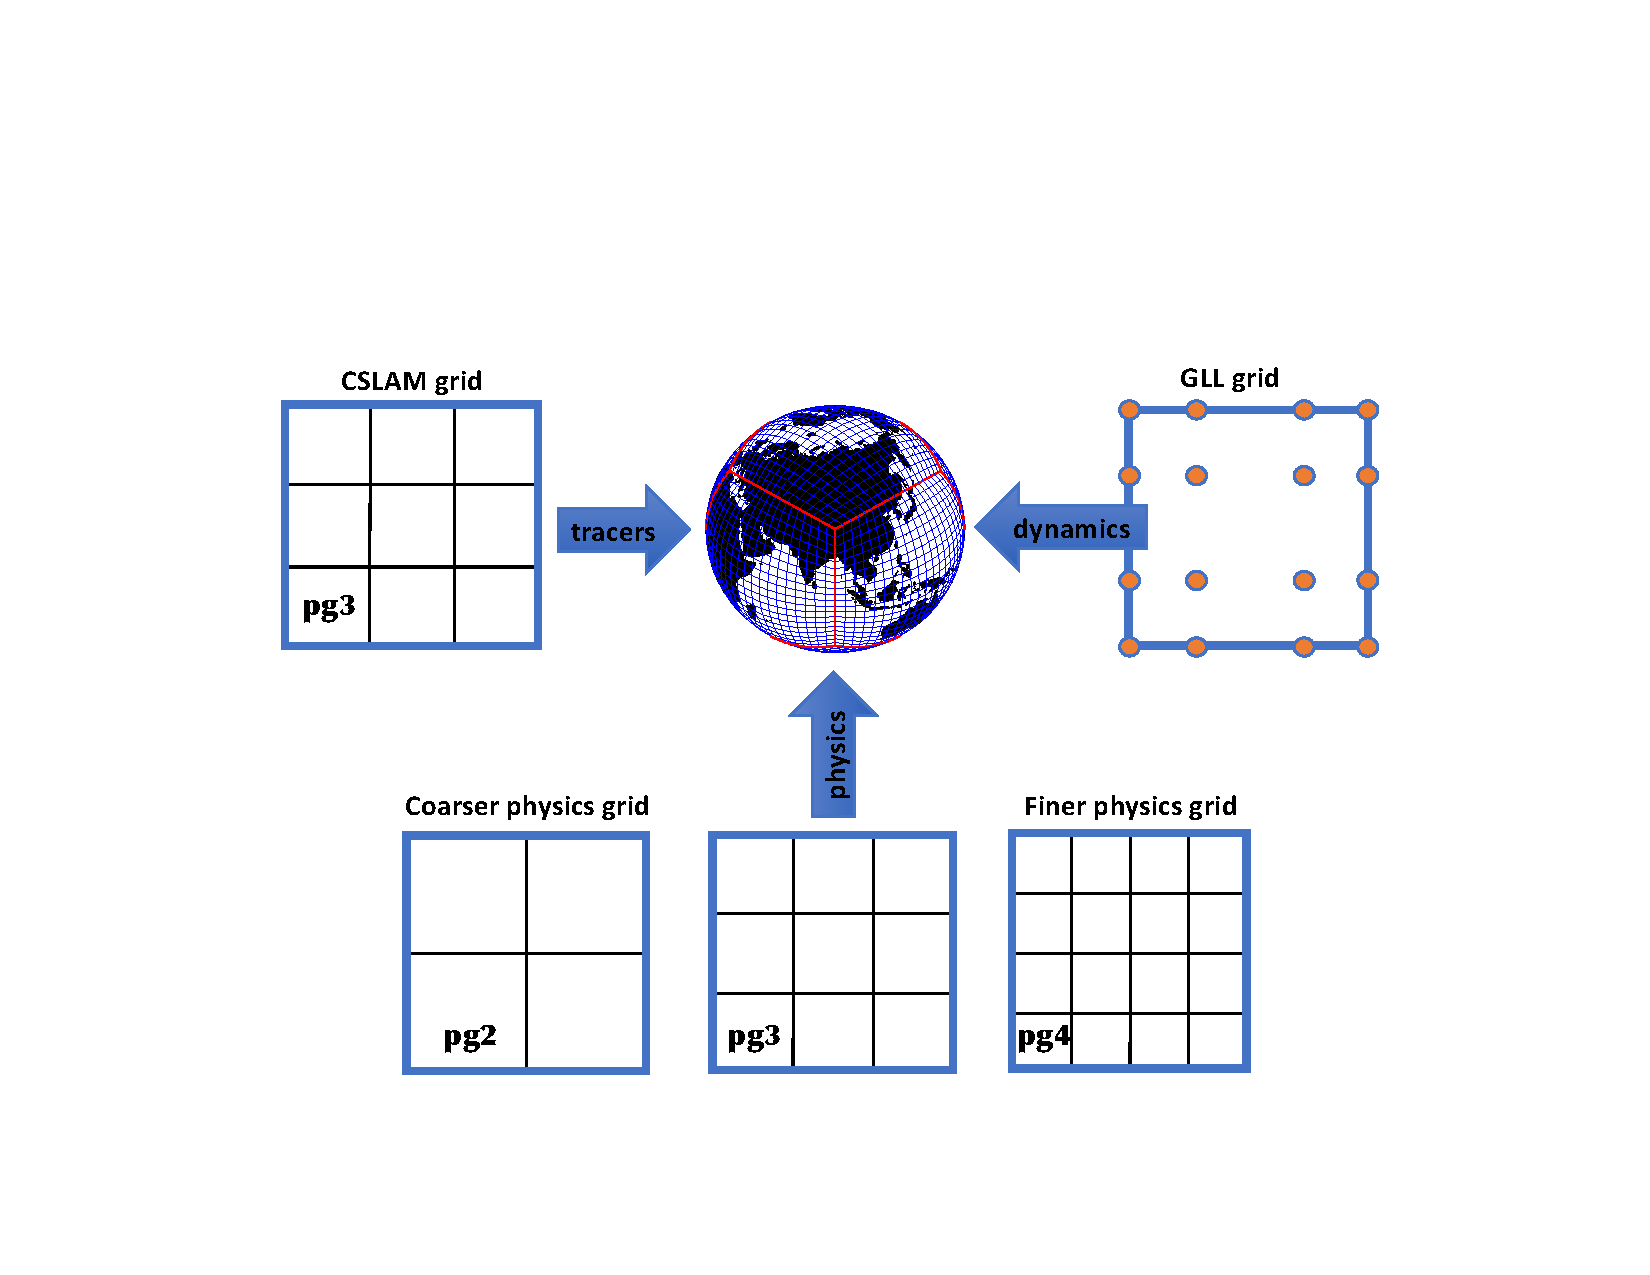
\includegraphics[width=30pc,angle=0]{figs/fig-overview.pdf}\\
\end{center}
\caption{An overview of the different grids in CAM-SE-CSLAM.}
\label{fig:overview}
\end{figure}

Similarly to the CAM-SE-CSLAM $pg3$ configuration, the dynamics state (momentum vector, temperature, dry pressure) must be mapped from the $GLL$ grid to the physics grid. Exactly the same algorithms as used in the $pg3$ configuration apply, i.e. momentum components are interpolated by evaluating the internal Lagrange basis functions (used in the spectral-element method) at the equi-angular (gnomonic) center of the $pg2$ cells and the Lagrange basis function representations of temperature and pressure are integrated over the $pg2$ control volumes. See H18 for details.

As compared to the $pg3$ configuration, the extra complication with the $pg2$ setup is that the tracer grid does not coincide with the physics grid, i.e. the tracer state needs to be mapped from the CSLAM grid ($pg3$) to the physics grid ($pg2$), and tracer increments computed by physics must be mapped from the physics grid back to the CSLAM grid. In order to describe the mapping algorithms between the grids some notation needs to be introduced.

The mapping algorithms are applied to each element $\Omega$ (with spherical area $\Delta \Omega$) so without loss of generality consider one element. Let $\Delta A^{(pg2)}_k$ and $\Delta A^{(pg3)}_\ell$ be the spherical area of the physics grid cell $A^{(pg2)}_k$ and CSLAM control volume $A^{(pg3)}_\ell$, respectively. The physics grid cells and CSLAM cells, respectively, span the element, $\Omega$, without gaps or overlaps
\begin{eqnarray}
\cup_{k=1}^{nphys^2}A^{(pg2)}_k=\Omega \text{ and } A^{(pg2)}_k \cap A^{(pg2)}_\ell = \emptyset \quad \forall k\ne \ell,\\
\cup_{k=1}^{nc^2}A^{(pg3)}_k=\Omega \text{ and } A^{(pg3)}_k \cap A^{(pg3)}_\ell = \emptyset \quad \forall k\ne \ell,
\end{eqnarray}
where $nc=3$ is the CSLAM grid resolution parameter and $nphys=2$ is the physics grid resolution parameter (following the Fortran code base), although the methods described here are valid for any arbitrary integer $nphys$ (e.g., $nphys=4$ is shown in Figure~\ref{fig:overview}). The overlap areas between the $k$-th physics grid cell and $\ell$th CSLAM cell are denoted
\begin{equation}
A_{k\ell}=A^{(pg2)}_k \cap A^{(pg3)}_\ell,
\end{equation}
(see Figure \ref{fig:area-schematic}) so that
\begin{equation}
A^{(pg2)}_k=\cup_{l=1}^{nc^2}A_{k\ell}.
\end{equation}
This overlap grid is also referred to as the {\em{exchange grid}}.
\subsection{Mapping tracers from $A^{(pg3)}$ to $A^{(pg2)}$ (CSLAM to physics grid)}\label{sec:nctopg}
The CSLAM and physics grids are both finite-volume grids so existing CSLAM technology can be used to map the tracer state from CSLAM to physics grid. That is, compute a high-order shape-preserving reconstruction of mixing ratio $m$ and dry air mass  $\frac{1}{g}\Delta p$ per unit area in each CSLAM control volume and integrate those reconstruction functions over the overlap areas \citep{LNU2010JCP,NL2010JCP}. This algorithm retains the properties of CSLAM: inherent mass-conservation, consistency (constant mixing ratio is preserved), mixing ratio shape-preservation and linear-correlation preservation.

\begin{figure}[t]
\begin{center}
\noindent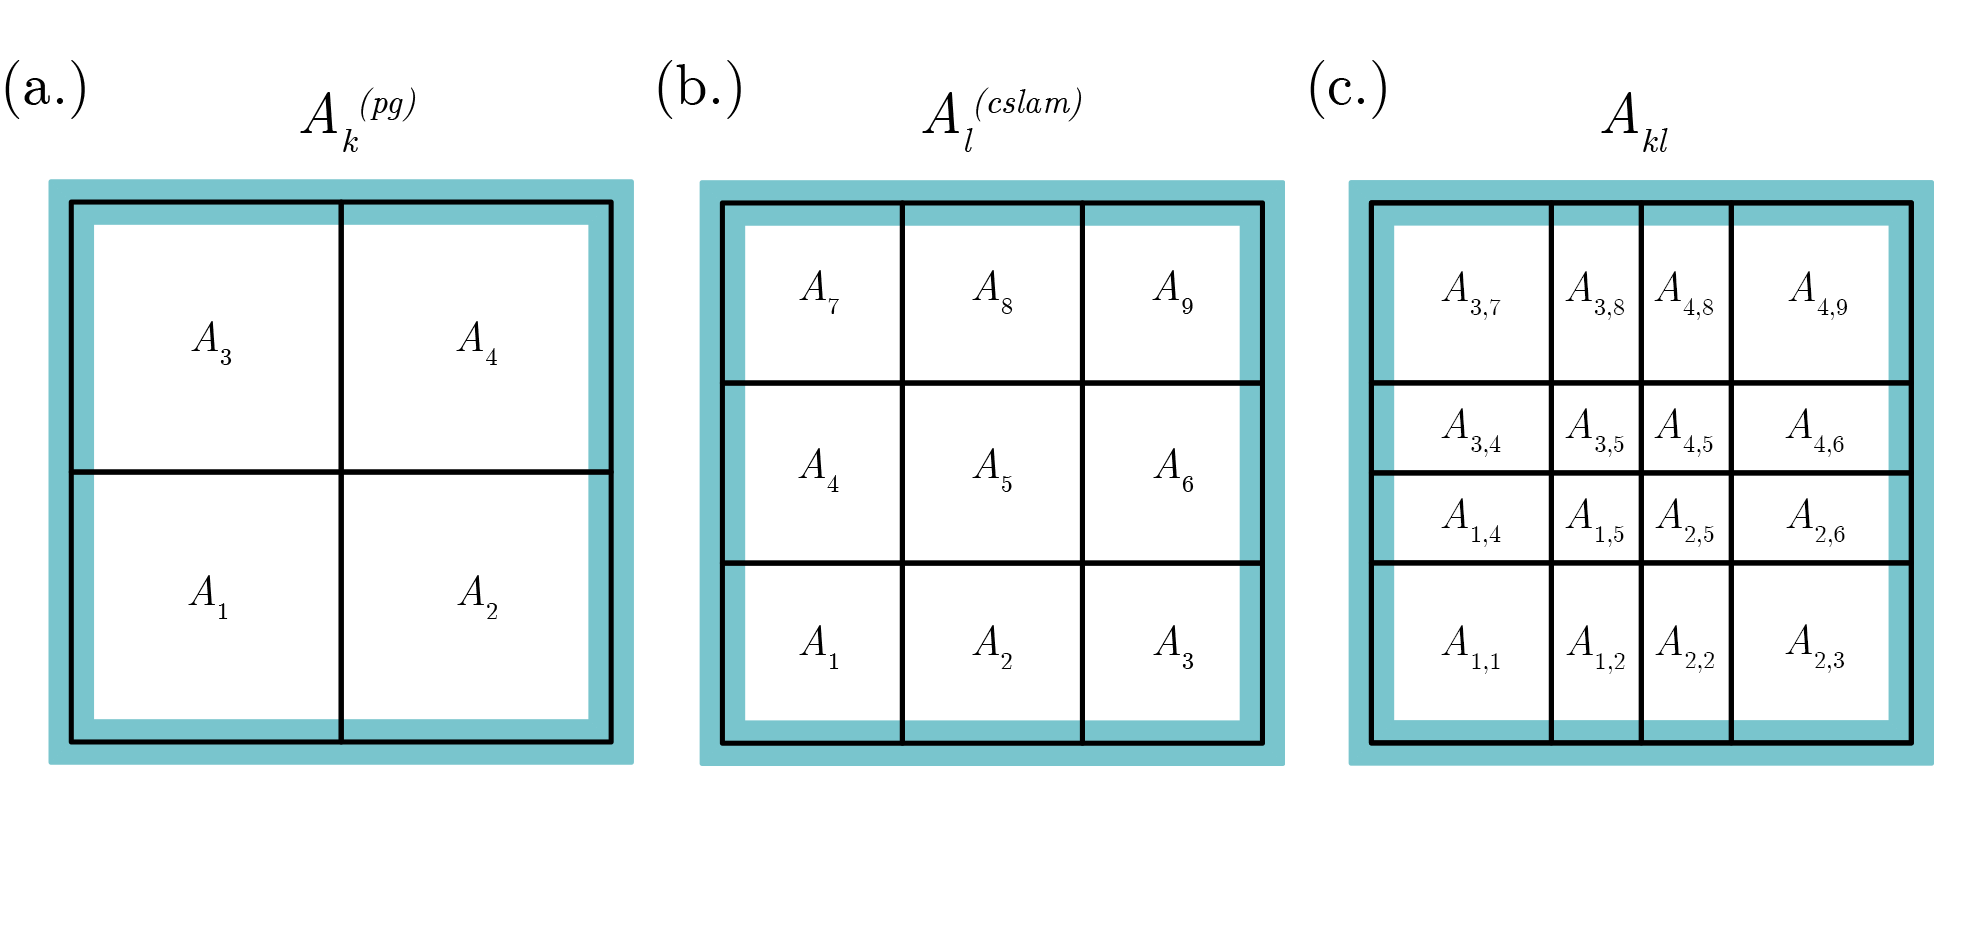
\includegraphics[width=30pc,angle=0]{figs/area-schematic.png}\\
\end{center}
\caption{Indices notation for (a) the $pg2$ grid, (b) the $pg3$ grid and (c) their exchange grid.}
\label{fig:area-schematic}
\end{figure}

Denote the known cell averaged values of dry pressure-level thickness and mixing ratio $\overline{\Delta p}^{(pg3)}$ and $\overline{m}^{(pg3)}$, respectively. We consider a particular layer and for simplicity drop the layer subscript. The same procedure is applied to each layer in a column. The unknowns we would like to compute is the cell-averaged values of the same quantities on the physics grid; $\overline{\Delta p}^{(pg2)}$ and $\overline{m}^{(pg2)}$, respectively. The dry pressure level thickness integrated over the $k$'th physics grid cell is given by
\begin{equation}
\label{eq:p}
\overline{\Delta p}^{(pg2)}_k=\frac{1}{\Delta A^{(pg2)}_k}\sum_{\ell=1}^{nc^2}\left<\delta p\right>_{k\ell},
\end{equation}
where $\left< \delta p\right>_{k\ell}$ is the dry mass in a layer over overlap area $A_{k\ell}$. It is computed by integrating a high-order (2D polynomial of degree 2) reconstruction of pressure-level thickness in each CSLAM cell over the overlap area $A_{k\ell}$
\begin{equation}
\label{eq:pg3dp}
\left< \delta p\right>_{k\ell}=\int_{A_{k\ell}}\left[ \sum_{i+j\le 2}{\mathcal{P}}^{(ij)}_\ell x^{i}y^{j}\right] dA.
\end{equation}
The reconstruction coefficients ${\mathcal{P}}^{(ij)}_\ell$ in CSLAM cell $\ell$ are computed from the cell average pressure level thicknesses on the CSLAM grid $\overline{\Delta p}^{(pg3)}$ and the numerical integration over overlap areas is done by line-integrals. The details of that is given in \cite{LNU2010JCP} and not repeated here.

The average tracer mass per unit area on the physics grid is given by
\begin{equation}
\label{eq:mp}
\overline{m\Delta p}^{(pg2)}_k=\frac{1}{\Delta A^{(pg2)}_k}\sum_{\ell=1}^{nc^2}\left< m\delta p\right>_{k\ell},
\end{equation}
where $\left< m\delta p\right>_{k\ell}$ is the tracer mass over $A_{k\ell}$ resulting from integrating a high-order reconstruction of $\Delta p$ and $m$ combined using the approach outlined in Appendix B of \cite{NL2010JCP} over the overlap area $A_{k\ell}$
\begin{equation}
\label{eq:mp2}
\left< m\delta p\right>_{k\ell}=\int_{A_{k\ell}}\left[ \overline{\Delta p}_\ell^{(pg3)}\sum_{i+j\le 2}{\mathcal{M}}^{(ij)}_\ell x^{i}y^{j}+{\overline{m}}_\ell^{(pg3)}\sum_{i+j\le 2}{\widetilde{{\mathcal{P}}}}^{(ij)}_\ell x^{i}y^{j}\right] dA,
\end{equation}
where ${\widetilde{{\mathcal{P}}}}^{(00)}_\ell={\mathcal{P}}^{(00)}_\ell-\overline{\Delta p}^{(pg3)}_\ell$ and ${\widetilde{{\mathcal{P}}}}^{(ij)}_\ell={\mathcal{P}}^{(ij)}_\ell$ for $i,j>0$, and ${\mathcal{M}}^{(ij)}_\ell$ are the reconstruction coefficients for the mixing ratio in CSLAM cell $A^{(pg3)}_\ell$. A shape-preserving limiter is applied to the reconstruction of mixing ratio $m$ \citep{BJ1989} and not $\Delta p$. This way of combining the reconstruction function for $\Delta p$ and $m$ in \eqref{eq:mp2} ensures that a constant mixing ratio is preserved (consistency), tracer mass is conserved, linear-correlations are preserved and tracer shape-preservation is retained. The mixing ratio on the physics grid is then
\begin{equation}
{\overline{m}}^{(pg2)}_k=\frac{\overline{\left( m\Delta p\right)}^{(pg2)}_k}{\overline{\Delta p}^{(pg2)}_k},
\end{equation}
where $\overline{\Delta p}^{(pg2)}_k$ is given in \eqref{eq:p}. 

Perhaps surprisingly a much more challenging problem is to map tracer increments (or state) from the physics grid to the CSLAM grid while retaining important properties such as mass-conservation, consistency, and correlation preservation. Why this mapping problem is challenging is explained in detail in Section \ref{sec:why} after having defined important properties for mapping physics increments/tendencies.
\subsection{Mapping tracer increments from $A^{(pg2)}$ to $A^{(pg3)}$ (physics to CSLAM grid)}\label{sec:pgtonc}
The increments from the parameterizations are computed on the physics grid. The tracer increment in physics grid cell $k$ is denoted $\overline{f}_k^{(pg2)}$ so that the updated mixing ratio on the physics grid is ${\overline{m}}^{(pg2)}_k+\overline{f}_k^{(pg2)}$. The problem is how to map $\overline{f}_k^{(pg2)}$ to the CSLAM control volumes, to obtain ${\overline{f}}^{(pg3)}$, satisfying the following constraints:
\begin{enumerate}
\item {\bf{Local mass-conservation}}: At a minimum total physics mass forcing on an element computed on the physics grid should equal the element physics mass forcing on the CSLAM grid
\begin{equation}
{\overline{f}}_k^{(pg2)}{\overline{\Delta p}}^{(pg2)}_k\Delta A_k^{(pg2)}=\sum_{\ell=1}^{nc^2}\left[{\overline{\Delta p}}^{(pg3)}_\ell {\overline{f}}^{(pg3)}_\ell\Delta A_{k\ell}\right],
\end{equation}
where $\overline{\Delta p}^{(pg2)}_k$ is the pressure level thickness in physics grid cell $k$ and similarly for $\overline{\Delta p}^{(pg3)}$. We enforce a more local constraint in which only mass-increments overlapping with a particular CSLAM cell contributes to the mass-increment in that CSLAM cell.
\item {\bf{Local shape-preservation in mixing ratio}}: The increments mapped to the CSLAM grid and added to the previous CSLAM state should not produce values smaller than the updated physics grid mixing ratios, ${\overline{m}}^{(pg2)}_k+\overline{f}_k^{(pg2)}$, or values smaller than the existing CSLAM mixing ratios that overlap with physics grid cell $A_\ell$
\begin{equation}
\label{eq:min}
\overline{m}^{(pg3)}_\ell+{\overline{f}}^{(pg3)}_\ell \ge \overline{m}^{(min)}_k=\min \left( {\overline{m}}^{(pg2)}_k+{\overline{f}}_k^{(pg2)},\left\{ {\overline{m}}_{k\ell} |\ell=1,nc^2\right\} \right),
\end{equation}
where
\begin{equation}
\label{eq:moverlap2}
\overline{m}_{k\ell}=\frac{\left< m\delta p_{k\ell}\right> }{\left< \delta p_{k\ell}\right>}.
\end{equation}
The nominator and denominator in \eqref{eq:moverlap2} are defined in \eqref{eq:pg3dp} and \eqref{eq:mp2}, respectively. In particular this means that an increment, when mapped to the $pg3$ grid, should not drive the state negative (described in detail below as the `negativity' problem).

A similar definition apply for maxima
\begin{equation}
\label{eq:max}
{\overline{m}}^{(pg3)}_\ell+{\overline{f}}^{(pg3)}_\ell \le \overline{m}_k^{(max)}=\max \left( {\overline{m}}^{(pg2)}_k+\overline{f}_k^{(pg2)},\left\{ {\overline{m}}_{k\ell} |\ell=1,nc^2\right\} \right),
\end{equation}
\item {\bf{Linear correlation preservation}}: The physics forcing must not disrupt linear tracer correlation between species on the CSLAM grid \citep[see, e.g., ][]{LT2011QJR}, i.e. if two tracers are linearly correlated and the physics increment preserves linear correlations on the physics grid then the tracer increment on the CSLAM grid must not disrupt linear correlations.
\item {\bf{Consistency}}: A non-zero constant mixing ratio increment from physics, $cnst$, on the physics grid, $\overline{f}_k^{(pg2)}=cnst$ $\forall k$, must result in the same (constant) forcing on the CSLAM grid, $\overline{f}_\ell^{(pg3)}=\overline{f}_k^{(pg2)}=cnst$ $\forall \ell$.
\end{enumerate}
To motivate the algorithm that will simultaneously satisfy 1-4 it is informative to discuss how `standard' mapping algorithms will violate one or more of the constraints:
\subsubsection{Why `conventional' conservative remapping will not work}\label{sec:why}
It is helpful to analyze in detail why conventional remapping can not satisfy properties 1-4 above. Assume that one remaps the mass-increments in exactly the same way as the mapping of mixing ratio state from the CSLAM grid to the physics grid described in section \ref{sec:nctopg}. That is, replace $m$ with $f$ and map from physics grid to the CSLAM grid instead of the other way around. Denote the mapped mass-increment $\widetilde{\overline{f\Delta p}}^{(pg3)}$ and due to the properties of the mapping algorithm the mass-increment is conserved, linear correlation between mass-increments are conserved and shape in mass-increment is preserved. The problems arise when converting from mass to mixing ratio.
\paragraph{Conserve mass but not consistency} 
If ones uses the known pressure-level thickness on the CSLAM grid ${\overline{\Delta p}}^{(pg3)}_k$ to convert from mass-increment to mixing-ratio increment
\begin{equation}
\label{eq:convert1}
\overline{m}^{(pg3)}_k=\frac{\widetilde{\overline{f\Delta p}}^{(pg3)}_k}{{\overline{\Delta p}}^{(pg3)}_k},
\end{equation}
a constant mixing ratio increment is not conserved. Basically the constant increment mapped to the CSLAM grid and converted to mixing ratio increment through \eqref{eq:convert1} will, rather than being constant, reflect the spurious discrepancy between $\widetilde{\overline{\Delta p}}^{(pg3)}_k$ and ${\overline{\Delta p}}^{(pg3)}_k$, where $\widetilde{\overline{\Delta p}}^{(pg3)}_k$ is the pressure-level thickness mapped from the $pg2$ grid to the $pg3$ grid. That said, mass will be conserved since the dynamical core state has ${\overline{\Delta p}}^{(pg3)}_k$ (unless the increment drives the mixing ratio negative - described in detail below). 
\paragraph{Consistent but not mass-conserving} 
Rather than converting to mixing ratio using ${\overline{\Delta p}}^{(pg3)}_k$, a constant increment can be preserved by using
\begin{equation}
\overline{m}^{(pg3)}_k=\frac{\widetilde{\overline{f\Delta p}}^{(pg3)}_k}{\widetilde{\overline{\Delta p}}^{(pg3)}_k},
\end{equation}
instead. But now mass-conservation is lost since, again, $\widetilde{\overline{\Delta p}}^{(pg2)}_k\ne {\overline{\Delta p}}^{(pg2)}_k$. This issue is similar to the mass-wind inconsistency found in specified dynamics applications \citep[e.g.][]{JKLSBCRE2001QJR,L2009LNCE}. 

\begin{figure}[t]
\begin{center}
\noindent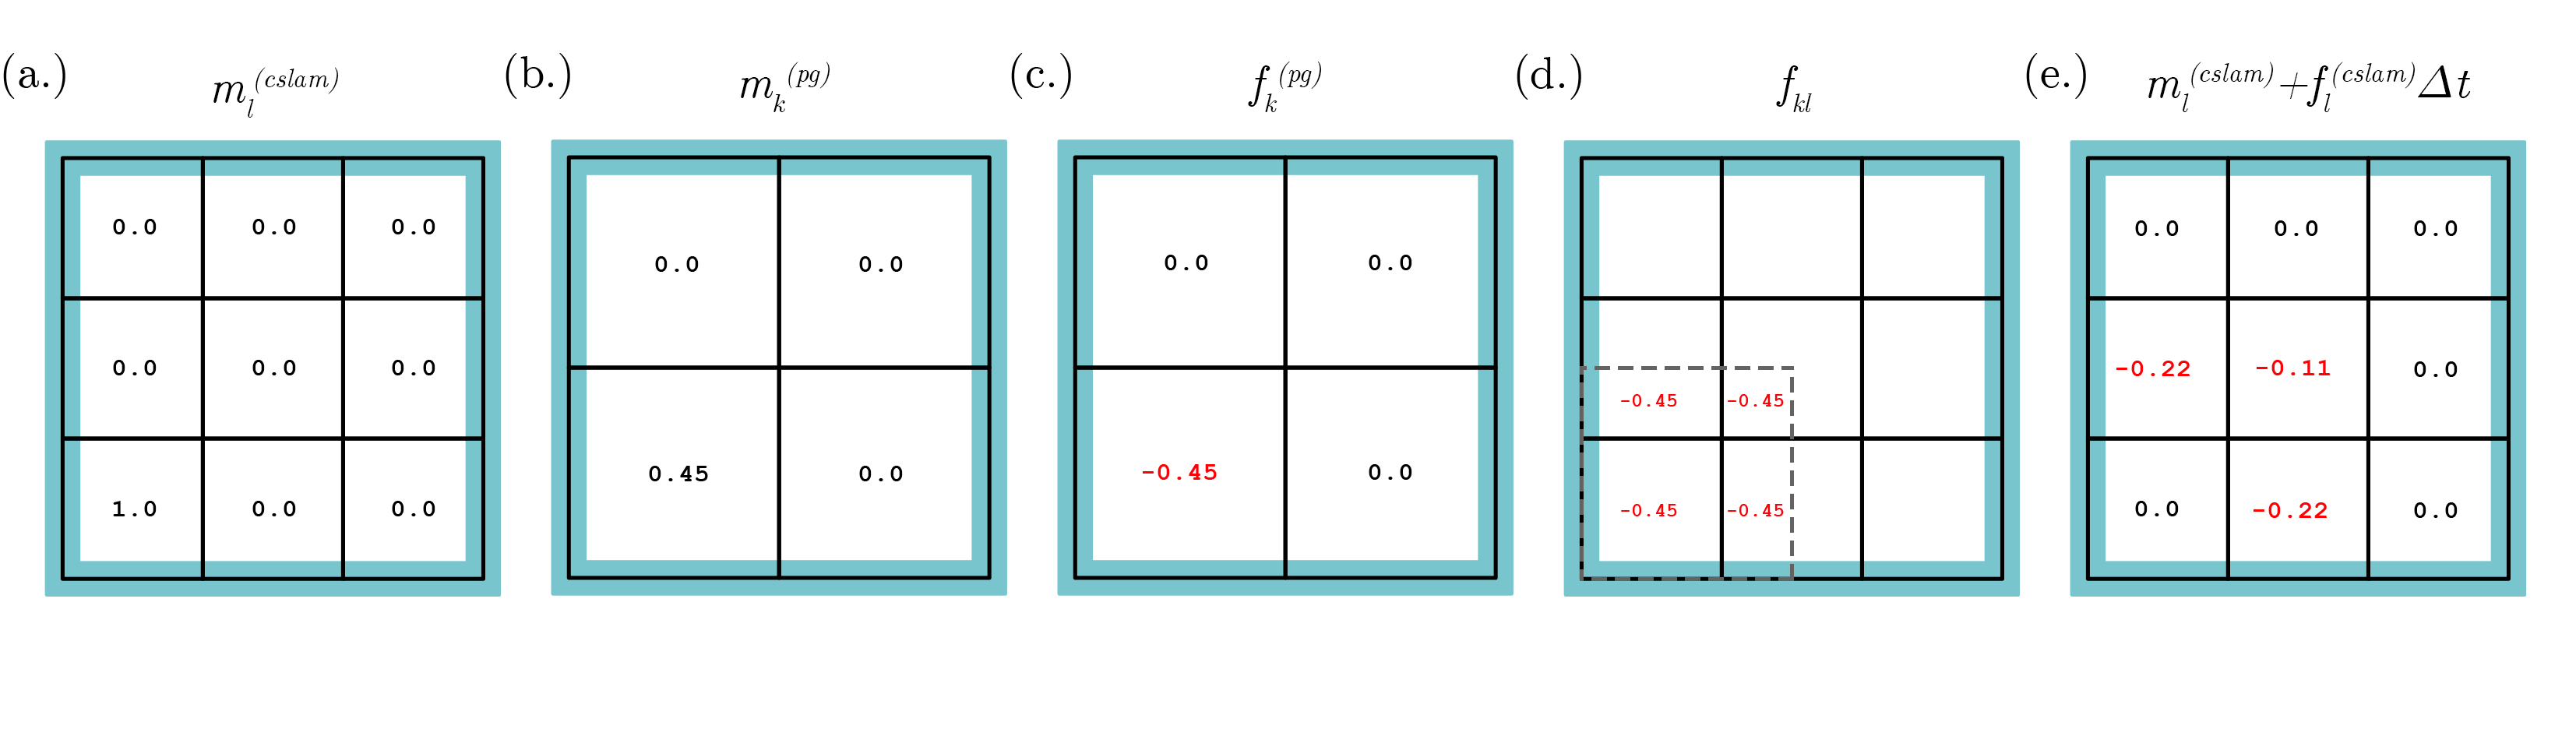
\includegraphics[width=30pc,angle=0]{figs/alg-schematic.png}\\
\end{center}
\caption{Schematic illustration of the `negativity problem' in a single element. (a.) Initial CSLAM tracer values, (b.) mapped to $pg2$, (c) produces a tracer increment on $pg2$, (d.) with negative increments on the exchange grid overlying CSLAM cells in (a) that were initially zero and (e) driving those mixing ratios negative.}
\label{fig:alg-schematic}
\end{figure}
\paragraph{The `negativity' problem and linear correlations} 
Even if one could derive a reversible map for mapping ${\overline{\Delta p}}^{(pg2)}$ from the physics grid to the CSLAM grid, there could still be problems if the increment drives the mixing ratios negative (or overshooting occurs) on the CSLAM grid. This can easily happen for tracers, such as cloud liquid amount and cloud ice amount, that are zero in most of the domain and non-zero in localized areas/points (where there are clouds). We refer to this as the `negativity problem'. This problem is depicted schematically in Figure~\ref{fig:alg-schematic}. Consider a single element of CSLAM control volumes, containing only a single cell with mixing ratio $1.0$, and $0.0$ everywhere else ($\overline{m}^{(pg3)}_\ell$; Figure ~\ref{fig:alg-schematic}a). The mixing ratios are mapped to the $pg2$ grid using, for simplicity, the piecewise constant method where a constant value inside the $pg2$ cells is used during the integration over overlap cells ($\overline{m}^{(pg2)}_k$; Figure~\ref{fig:alg-schematic}b). Now consider the case in which physics removes all the mass from the physics cell $k$: $\overline{f}^{(pg2)}_k=-\overline{m}^{(pg2)}_k$ (Figure~\ref{fig:alg-schematic}c). The tracer increment is mapped from $pg2$ to $pg3$ using the piecewise constant method. Some of the non-zero increments are now in overlap areas where the original CSLAM grid cells have mixing ratio zero ($\overline{f}_{k\ell}$; Figure~\ref{fig:alg-schematic}d), and hence, the state is driven negative when adding the overlap increment to the CSLAM state (Figure~\ref{fig:alg-schematic}e).  This is referred to as the negativity problem although it can also happen for maxima.

The negativity issue could be avoided if one remaps the physics updated state instead of mapping increments/tendencies. In that case a shape-preserving filter will make sure that the state on the CSLAM grid is not negative (and does not overshoot). That said, if physics does not change the state and it is mapped back to the CSLAM grid then spurious tendencies (proportional to the errors introduced by mapping state from the CSLAM grid to the physics grid and back again) are introduced. Hence it is advantageous to map increments/tendencies since any reasonable algorithm will preserve a zero function.

%In the $pg2$ configuration, mapping the fields to and from the quadrature grid and $pg2$ grid is identical to that described in H18. As discussed above above, in mapping to the physics grid, CAM-SE's Lagrange basis functions are integrated over the $pg2$ control volumes to provide the physics with a volume averaged state. The procedure is accurate to machine precision, conserves thermal energy and dry air mass, and is consistent (i.e., the mapping preserves a constant). The reverse mapping, from the physics grid to the quadrature grid, is done using a tensor-product Lagrange interpolation (see Appendix A in H18). The Lagrange interpolation is consistent, conserves dry air mass ({\color{red}{Peter, is this true?}}), but does not conserve thermal energy. Errors arising from the lack of energy conservation were estimated to be small; about two orders of magnitude less than the energy dissipation due to the dynamical core alone.

%The semi-Lagrangian advection of tracers in our $pg2$ configuration is solved on the CSLAM grid. 





%Interpolation: Traditional Lagrange interpolate of the mixing ratio increment would preserve a constant and could be made shape-preserving using {\em{ad hoc}} filters \citep[e.g.][]{BC2002MWR} but will not inherently preserve mass increment and suffers from the `negativity problem' described above.

As illustrated above a standard remapping method will NOT simultaneously satisfy 1-4 and hence a new algorithm has been derived.
\subsection{New tendency mapping algorithm}\label{sec:massfix}
Although this algorithm is explained and examined for a $pg2$ grid, it is general for any $pgX$ resolution. The problem is how to map the mass-increment on the physics grid, ${\overline{f}}^{(pg2)}\Delta A^{(pg2)}$, to the CSLAM cells that overlap with $\Delta A^{(pg2)}$. To maintain shape-preservation, linear correlations and to avoid the negativity problem locally, it is advantageous to define a mass excess function on the exchange grid $\Delta m_{k\ell}^{(excess)}$. It is basically the maximum amount of mixing ratio that can be removed (in the case ${\overline{f}}^{(pg2)}<0$) without producing new minima in the exchange grid mixing ratio $m_{k\ell}$
\begin{equation}
\Delta m^{(excess)}_{k\ell}=\overline{m}_{k\ell}-\overline{m}_k^{(min)},
\end{equation}
where $\overline{m}_{k\ell}$ is defined in \eqref{eq:moverlap2}. So the maximum amount of mass that we can be removed from the exchange grid cells that span physics grid cell $A_k$ without violating the shape-preservation constraint (\eqref{eq:min} and \eqref{eq:max}) is
\begin{equation}
\sum_\ell \Delta m^{(excess)}_{k\ell}\overline{\Delta p}_{k\ell} \delta A_{k\ell}.
\end{equation}
If physics is designed not to remove more mass than available in $A_k$ (which should be the case for a carefully designed physics package) then it is guaranteed that
\begin{equation}
\label{eq:well-posed}
\sum_\ell \Delta m^{(excess)}_{k\ell}\overline{\Delta p}_{k\ell} \delta A_{k\ell}\ge {\overline{f}}^{(pg2)}\Delta p_k\Delta A^{(pg2)}.
\end{equation}
We distribute the physics mass-forcing (assuming ${\overline{f}}^{(pg2)}<0$) according to the mass excess in each overlap area by solving this equation for $\gamma_k$
\begin{equation}
\label{eq:mass-excess}
\Delta A_k^{(pg2)}\overline{\Delta p}_k^{(pg2)}{\overline{f}}^{(pg2)}=\gamma_k \sum_\ell \Delta m^{(excess)}_{k\ell}\overline{\Delta p}_{k\ell} \delta A_{k\ell},
\end{equation}
and add mass increment (which in this case is negative)
\begin{equation}
\label{eq:mass-incr}
\gamma_k \Delta m^{(excess)}_{k\ell}\overline{\Delta p}_{k\ell} \delta A_{k\ell},
\end{equation}
to the $\ell$th CSLAM cell state ${\overline{m}}^{(pg3)} \overline{\Delta p}^{(pg3)}_\ell \Delta A^{(pg3)}_\ell$. This process is repeated for all physics cells. Note that this problem is a well-posed, i.e. $\gamma_k>0$, since physics will not remove more mass than is locally available \eqref{eq:well-posed}. The way in which the mass-forcing is distributed to the CSLAM cells using the excess function insures that the negativity problem is avoided. Mass is conserved by design and shape-preservation is obtained by using the excess function.

If the physics increment is positive (assuming ${\overline{f}}^{(pg2)}>0$) we define a `lack' function
\begin{equation}
\Delta m^{(lack)}_{k\ell}=\overline{m}_{k\ell}-\overline{m}^{(max)},
\end{equation}
and solve
\begin{equation}
\label{eq:mass-lack}
\overline{\Delta p}_k^{(pg2)}{\overline{f}}^{(pg2)}\Delta A_k^{(pg2)}=\gamma_k \sum_\ell \left[ \Delta m^{(lack)}_{k\ell}\overline{\Delta p}_{k\ell} \delta A_{k\ell}\right],
\end{equation}
for $\gamma_k$ and follow the same procedure as for mass excess. Since positive and negative forcing is treated in exactly the same way, linear correlations are preserved. Note how the definition of the excess/lack function insures linear correlation preservation; for example, if one would prevent negative values and not do anything about overshoots then linear correlations would not be preserved since the minima and maxima are not treated in the same way.

While the above algorithm satisfies properties 1-4 in section \ref{sec:pgtonc}, it is not a high-order algorithm in terms of formal accuracy. This is illustrated in Figure \ref{fig:mapping} (row 3) where a smooth analytical tendency \citep[approximate spherical harmonic of order 32 and azimuthal wave number 16; ][]{J1999MWR}
\begin{equation}
\label{eq:Y32}
f^{(pg2)}=\frac{1}{2}+\frac{1}{2}\cos(16\lambda)\sin(2\theta)^{16},
\end{equation}
where $(\lambda,\theta)$ is latitude-longitude, is mapped from $pg2$ to $pg3$ grid using this algorithm assuming $m^{(pg3)}_\ell=0, \quad \forall \ell$. The errors in the mapping are not always aligned with large gradients in the analytical function as would be expected for a `traditional' interpolation algorithm. The errors are maximum on the order of 60$\%$. To reduce errors we therefore perform a higher-order pre-allocation of tendencies that is not mass-conserving but satisfies properties 2,3, and 4 in Section \ref{sec:pgtonc}.

\begin{figure}[t]
\begin{center}
\noindent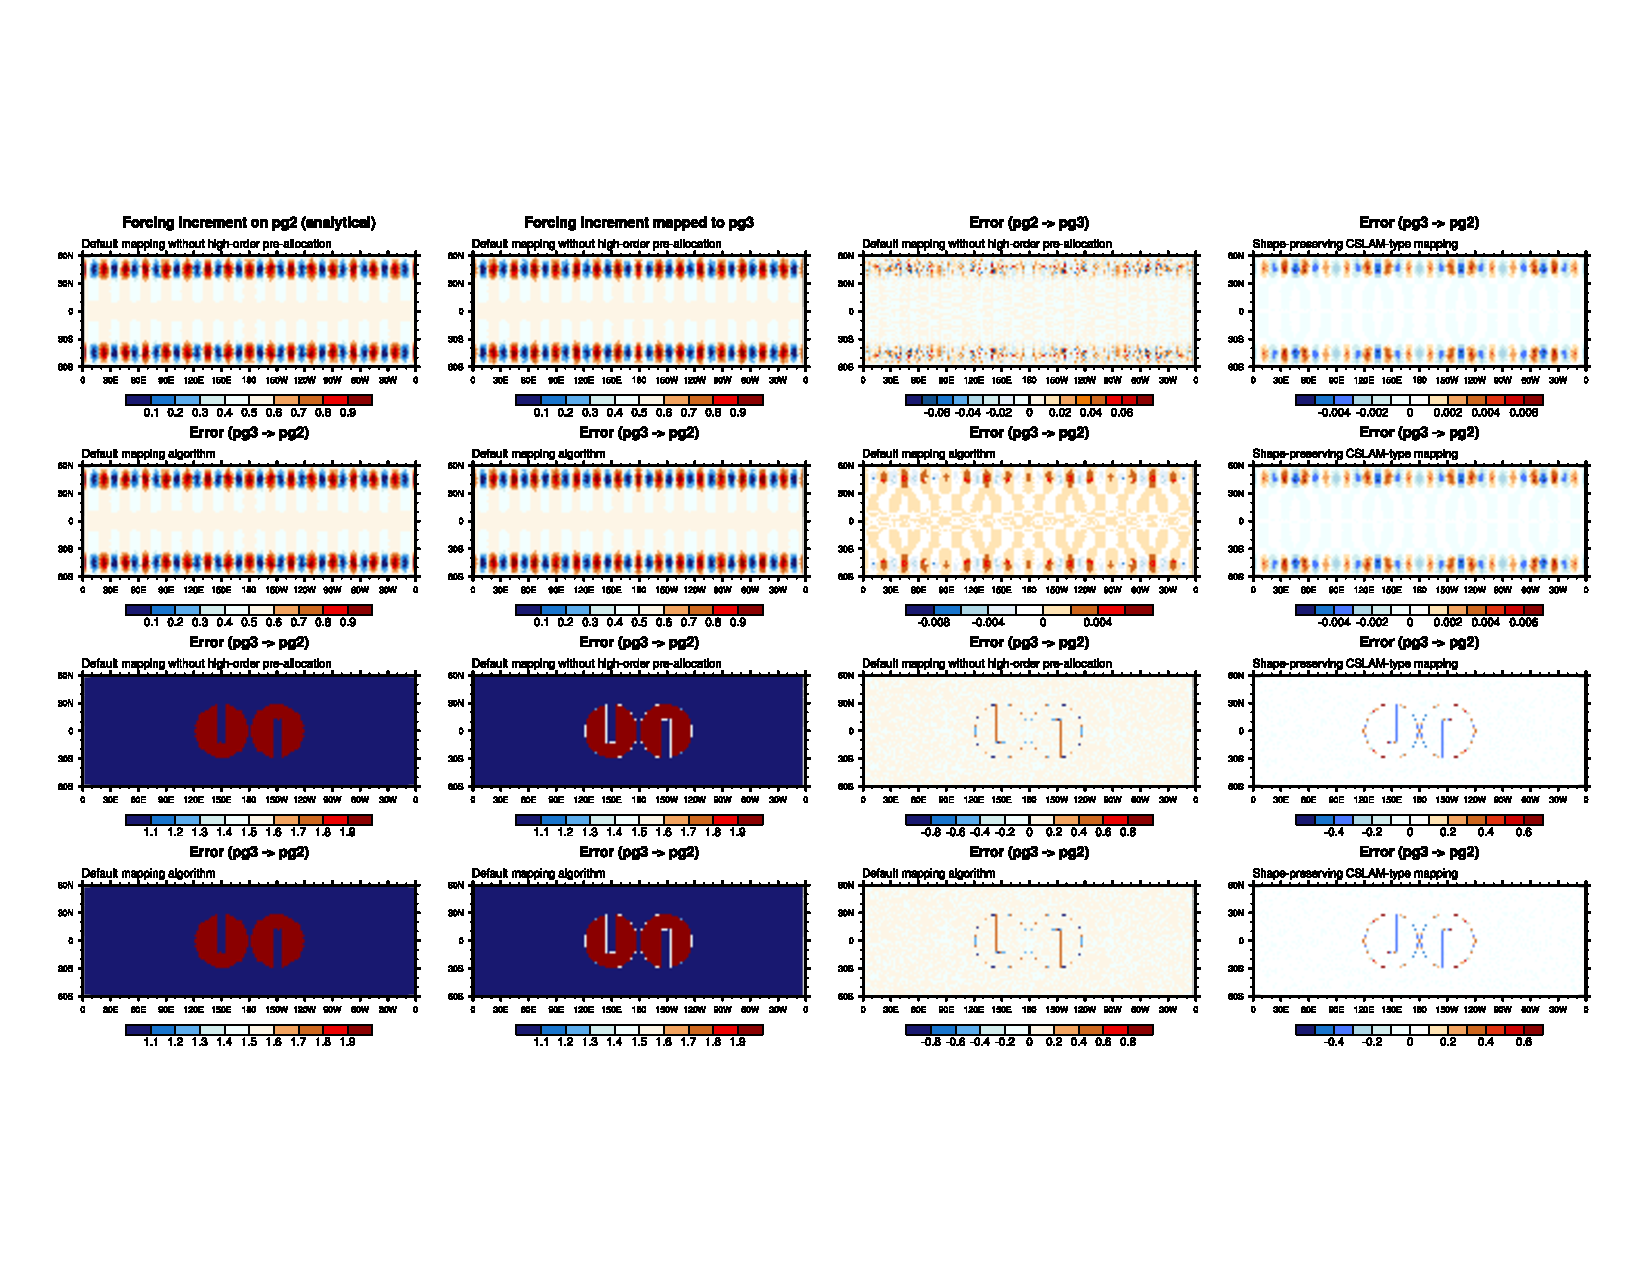
\includegraphics[width=30pc,angle=0]{figs/mapping.pdf}\\
\end{center}
\caption{Mapping of idealized functions from $pg2$ (column 1) to $pg3$ (columns 2) and errors (column 3) using the new tendency algorithm only (row 1 and 3) and new tendency algorithm with the high-order pre-allocation (row 2 and 4). Column 4 shows the errors in mapping the same distributions from  $pg3$ to $pg2$ using traditional remapping (CSLAM technology).}
\label{fig:mapping}
\end{figure}

%Similarly we define a mass lack function

%which is the maximum amount of mixing ratio that can be added without creating new maxima.

\subsection{High-order (non-conservative) pre-allocation of tracer tendencies}
A high-order tracer mass increment in overlap area $A_{k\ell}$ can be computed using the following formula
\begin{equation}
\label{eq:mp3}
\left< f\delta p\right>_{k\ell}=\int_{A_{k\ell}}\left[ \overline{\Delta p}_\ell^{(pg3)}\sum_{i+j\le 2}{\mathcal{F}}^{(ij)}_k x^{i}y^{j}+{\overline{f}}_k^{(pg2)}\sum_{i+j\le 2}{\widetilde{{\mathcal{P}}}}^{(ij)}_\ell x^{i}y^{j}\right] dA,
\end{equation}
where $\mathcal{F}^{(ij)}_k$ is the forcing increment reconstruction coefficients in the $k$th physics grid cell and ${\overline{f}}_k^{(pg2)}$ is the average physics increment in the $k$th physics grid cell. Note that we are using the known dry pressure reconstruction coefficients on the $pg3$ grid instead of reconstructing sub-grid-scale pressure variations from the physics grid cell averaged values. We can do that since the dry pressure is not modified by physics. This highlights the importance of a dry-pressure formulation of the dynamical core when separating physics and dynamics grids \citep{LetAl2018JAMES}. If the physics forcing is constant then $\left< f\delta p\right>_{k\ell}$ exactly equals $\left<\delta p\right>_{k\ell}$ from \eqref{eq:pg3dp}; in other words, the mapping is designed to be reversible in dry pressure. The physics increment in terms of mixing ratio change is given by
\begin{equation}
\label{eq:pg3fq}
\overline{f}_{k\ell}=\frac{\left< f\delta p\right>_{k\ell}}{\left<\delta p\right>_{k\ell}},
\end{equation}
where the denominator is given by \eqref{eq:pg3dp}.

Shape-preservation, as defined by \eqref{eq:min} and \eqref{eq:max}, is enforced by eliminating under and overshoots on the exchange grid by modifying the forcing increment $\overline{f}_{k\ell}$ so that shape-preservation is not violated in the overlap areas{\footnote{In the computation of $\overline{m}_{k\ell}$ there can be small overshoots and undershoots (due to numerical integration errors) compared to the CSLAM cell average values $\overline{m}^{(pg3)}_\ell$ that it overlaps with so we set
\begin{equation}
\overline{m}_k^{(min)}=\min \left( \overline{m}_k^{(min)},\left\{ \overline{m}^{(pg)}_\ell)|\ell=1,nc^2\right\} \right)
\end{equation}}}
\begin{equation}
\overline{m}_k^{(min)} \le \overline{m}_{k\ell}+\widetilde{\overline{f}}_{k\ell} \le \overline{m}_k^{(max)}.
\end{equation}
While this algorithm preserves linear correlations, shape, and is consistent, is it not mass-conservative. Hence the remaining physics increment not allocated in the algorithm above is allocated using the new tendency algorithm described in Section \ref{sec:massfix}.

Combining the high-order pre-allocation algorithm with the new tendency algorithm (which in this case can also be considered as a mass-fixer that does not disrupt correlation-preservation, shape and consistency) leads to an order-of-magnitude reduction in mapping errors for a smooth function (see Figure \ref{fig:mapping} row 3 and 4) while full-filling the mass-conservation, shape-preservation, linear correlation and consistency  constraint. Mass and linear correlation preservation is illustrated in the baroclinic wave test with terminator chemistry test in Section \ref{sec:fkessler}. Shape-preservation and consistency is demonstrated in an idealized mapping test where a smooth function, see \eqref{eq:Y32}, and a slotted-cylinder \citep[see equation 12 in ][]{LSPT2012GMD} are mapped to/from the $pg2$ and $pg3$ grids. Since the background value in the mapping of the slotted-cylinder field is preserved the mapping algorithm is consistent. Since no new over- and undershoots are produced (particularly obvious in the mapping of the slotted cylinders) the mapping is shape-preserving. We also note that the mapping errors with the default algorithm (higher-order pre-allocation with new tendency algorithm) are similar to the errors in mapping the same field from $pg3$ to $pg2$ using traditional remapping with CSLAM technology (column 4 in Figure \ref{fig:mapping}).


%A high-order estimate of the physics increment in the $A_{k\ell}$th overlap cell, that is not mass-conserving, can be computed as
%\begin{equation}
%\label{eq:mp3}
%\overline{f}_{k\ell}=\frac{1}{\delta A_{k\ell}}\int_{A_{k\ell}}\left[ \sum_{i+j\le 2}{\mathcal{F}}^{(ij)}_k x^{i}y^{j}\right] dA,
%\end{equation}
%where $\mathcal{F}^{(ij)}_k$ are the recontruction coefficients for the physics increment $f$ in the $k$th physics grid cell. For reasons that will become clear a shape-preserving limiter is not applied when computing $\mathcal{F}^{(ij)}_k$. Each overlap increment is added to the CSLAM opverlap state $\overline{m}_{k\ell}$ 
%\begin{equation}
%\overline{m}_{k\ell}+\tilde{\overline{f}}_{k\ell},
%\end{equation}
%where $\tilde{\overline{f}}_{k\ell}$ is $\overline{f}_{k\ell}$ `cropped' so that shape-preservation is not violated locally


\section{Results}

A plethora of grids are developed for CAM-SE-CSLAM (Table \ref{table:grids}), and used to understand the sensitivity to physics grid resolution, across a wide range of spectral-element grid resolutions. The physics time-step, $\Delta t_{phys}$, used for each grid is scaled by the dynamics time-step to prevent time truncation errors at higher resolutions \citep{HR2018JAMES}. A hierarchy of idealized model configurations are presented (avialble in CESM2.0; \url{https://doi.org/10.5065/D67H1H0V}) to illuminate the differences between $pg2$ and $pg3$.

 \begin{table}
 \caption{Average equatorial grid spacing, $\Delta x$, and model time-step, $\Delta x$, used by the physical parameterizations, $phys$, and dynamical core, $dyn$.}
 \centering
 \begin{tabular}{llcccc}
 \hline
 Grid name & $\Delta x_{dyn}$  & $\Delta t_{dyn}$ & $\Delta x_{phys}$  & $\Delta t_{phys}$ \\
 \hline
   {\tt{ne}}20{\tt{pg3}}  & 166.8km & 300s  & 166.8km & 1800s \\
   {\tt{ne}}30{\tt{pg2}}  & 111.2km & 300s  & 166.8km & 1800s \\
   {\tt{ne}}30{\tt{pg3}}  & 111.2km & 300s  & 111.2km & 1800s \\
   {\tt{ne}}40{\tt{pg3}}  &  83.4km & 150s  &  83.4km &  900s \\
   {\tt{ne}}60{\tt{pg2}}  &  55.6km & 150s  &  83.4km &  900s \\
   {\tt{ne}}60{\tt{pg3}}  &  55.6km & 150s  &  55.6km &  900s \\
   {\tt{ne}}80{\tt{pg3}}  &  41.7km &  75s  &  41.7km &  450s \\
   {\tt{ne}}120{\tt{pg2}} &  27.8km &  75s  &  41.7km &  450s \\
   {\tt{ne}}120{\tt{pg3}} &  27.8km &  75s  &  27.8km &  450s \\
 \hline
 %\multicolumn{2}{l}{$^{a}$Footnote text here.}
 \end{tabular}
 \label{table:grids}
 \end{table}

\subsection{Moist Baroclinic Wave}

{\color{red}Terminator Test of linear-correlation preservation, and tracer mass conservation (just a number showing to within machine precision).}

\subsection{Held-Suarez with Topography}

Flow over rough topography may facilitate significant grid imprinting using the spectral element method \citep{gmdd-8-4623-2015,HL2018MWR}. A Held-Suarez configuration, modified with real world topography is used to identify grid imprinting over mountainous terrain. Figure \ref{fig:fhs-contours} (middle panel) shows the climatological mean vertical pressure velocity, $\omega$, over the Andes and Himalayan region and at two different levels in the mid-troposphere, using the $ne30pg3$ grid. All Held-Suarez simulations are ran for two-years. The figure is displayed as a raster plot on the native physics grid, so that indidual extrema, which characterize the flow over the Andes between about $10^\circ-20^\circ$ S, may be identified as spurious. Similarly, at the foot of the Himalayas, their appears to be spurious oscillatory bands of upward and downward motion aligned with the element boundaries. 

\begin{figure}[t]
\begin{center}
\noindent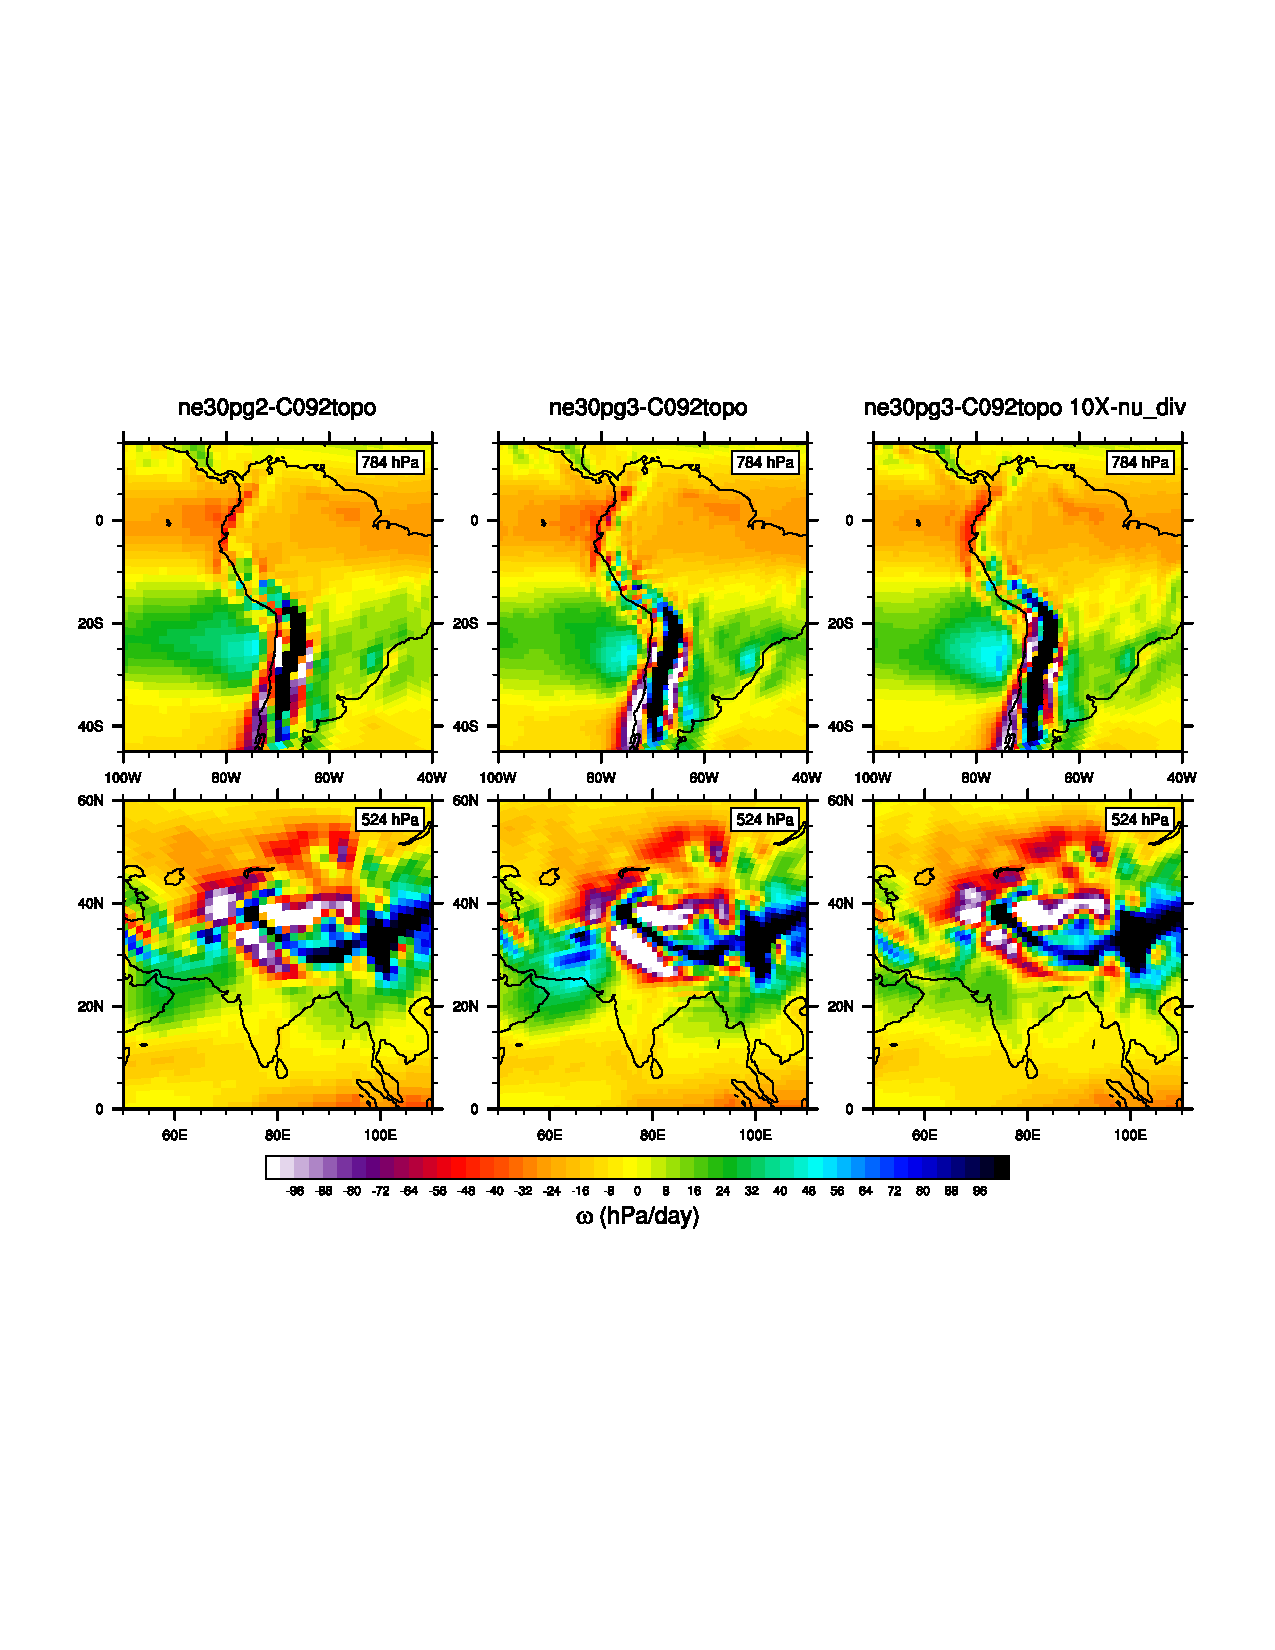
\includegraphics[width=30pc,angle=0]{figs/fhstopo_ne30pg2-v-ne30pg3-v-10Xnudiv.pdf}\\
\end{center}
\caption{Mean $\omega$ at two model levels in the middle troposphere, in a Held-Suarez configuration outfitted with real world topography. (Left) $ne30pg2$ (Middle) $ne30pg3$ and (Right) $ne30pg3$ with the divergence damping coefficient increased by an order of magnitude. The $\omega$ fields are computed a two-year simulation. The data are presented on a raster plot in order to identify individual grid cells}
\label{fig:fhs-contours}
\end{figure}

As discussed in \cite{HL2018MWR}, grid imprinting over the mountains tends to occur in regions of weak stability, and the extrema often  manifest as full tropsphere upward/downward couplets. Thus, grid imprinting over mountains can be alleviated through increasing the divergence damping in the model. Figure \ref{fig:fhs-contours} (right panel) repeats the $ne30pg3$ simulation, but increasing the divergence damping coefficient by an order of magnitude. The spurious noise over the Andes and the Himalayas are damped, as grid point extrema tends to be diffused into neighboring grid cells. The wave number-power spectrum of the kinetic energy arising from divergent modes is provided in Figure \ref{fig:fhs-div}, indicating that divergent modes are significantly damped at higher wavenumbers relative to the default $ne30pg3$ simulation. Requiring the divergence damping coefficient to be an order of magnitude larger than that required for numerical stability is not ideal from a model development perspective. The hyper-viscosity coefficients are one of the only free-parameters in the dynamical core to tune the kinetic energy spectrum to observations \citep{SPKS2014JAS,LetAl2018JAMES}.

\begin{figure}[t]
\begin{center}
\noindent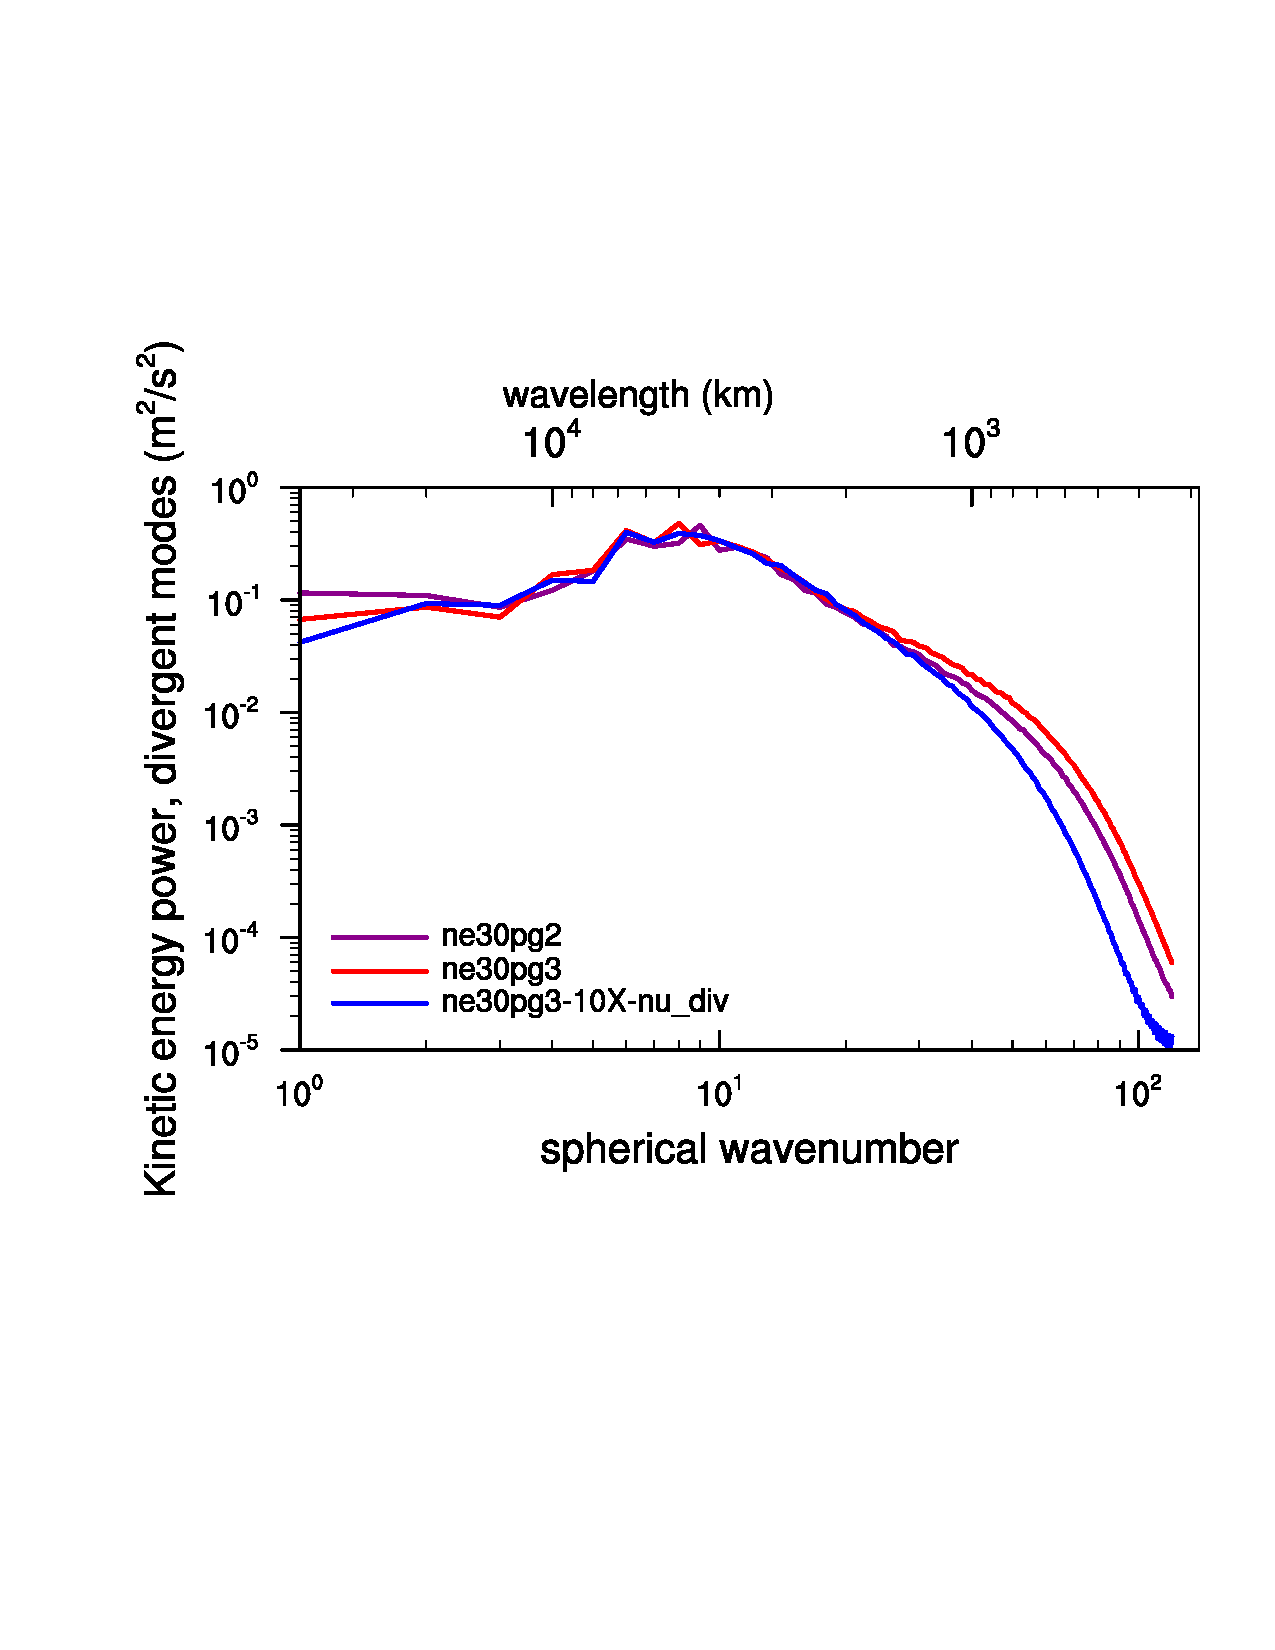
\includegraphics[width=25pc,angle=0]{figs/fhstopo_Divergence_ne30pg2-v-ne30pg3-v-10Xnudiv.pdf}\\
\end{center}
\caption{Kinetic energy power spectrum arising from divergent modes in $ne30pg2$, $ne30pg3$ and $ne30pg3$ with the divergence damping coefficient increased by an order of magnitude ($ne30pg3-10X-ne\_div$).}
\label{fig:fhs-div}
\end{figure}

The $\omega$ field in a $ne30pg2$ simulation is provided in Figure \ref{fig:fhs-contours} (left panel). Grid cell extrema over the Andes is less prevalent than in the $ne30pg3$ simulation, as seen by the reduction in large magnitude $\omega$ (red grid cells). The spurious oscillations at the foot of the Himalayas appears to have been entirely eliminated. This improvement in grid imprinting is due to the homogenization of nodal types in the $pg2$ configuration discussed in Section \ref{}. The divergent modes are slightly damped relative to the $ne30pg3$ simulations, almost sytematically with wavenumber, and much less than the simulation using the larger divergence damping coefficient (Figure \ref{fig:fhs-div}).  

\subsection{Aqua-planets}

The results of the previous section are consistent with our hypothesis, that spurious noise is effectively reduced, and visibly eliminated using a $pg2$ grid. We now turn to the question of whether the coarser resolution physics grid has an impact on the resolved scales of motion. This analysis will make use of an aqua-planet configuration \citep{NH2000ASL,MWO2016JAMES}; an ocean covered planet in perpetual equinox, and fixed, zonally-symmetric sea surface temperatures idealized after present day Earth. The aqua-planets are run for one simulated year, using CAM, version 6 physics (CAM6; $QPC6$ compset in CESM2.0).

\cite{HR2017JCLIM} has shown that through assuming the horizontal scale of the Archimedean buoyancy is linearly proportional to the grid spacing, the magnitude of the vertical motion in a set of aqua-planet runs did not scale like the inverse of the grid-spacing across a set of grid resolutions. However, the results of \cite{HR2018JAMES} indicate that the scaling may be recovered through a more judicous choice of $\Delta t_{phys}$ (Table \ref{table:grids}). To test this idea, three aqua-planet simulations are carried out using the $ne30pg3$, $ne60pg3$ and $ne120pg3$ grids. 

Figure \ref{fig:pg3panel}a shows the wave-number-power spectrum of the moist physics temperature tendencies (referred to as {\em{forcing}} throughout this study) in the upper troposphere, where statiform heating is common due to detrainment by the deep-convection scheme \citep{ZM1995AO}. There is a clear reduction in forcing scale with resolution, which is consistent with the increased magnitude of $\omega$ with resolution, expressed by the probability density distribution (PDF) of upward $\omega$, everywhere in the model (Figure \ref{fig:pg3panel}b). The PDFs may be scaled to the $ne120pg3$ grid using the scaling of \cite{PG2006JAS}, 
\begin{equation}
P(\omega_{s}) = \alpha \times P(\omega/\alpha),
\end{equation}
where $P(\omega_{s})$ is the PDF of the scaled $\omega$, $\omega_{s}$, and $\alpha$ is the ratio of the vertical velocity scale to the vertical velocity scale of the target grid resolution, set to $\alpha = \Delta x_{target}/\Delta x$, after \citep{HR2018JAMES}, where $\Delta x$ is the grid spacing and $\Delta x_{target}$ is the grid spacing of the target resolution. The scaled PDFs do not line up perfectly on top one another (Figure \ref{fig:pg3panel}c), but the scaling explains the change in magnitude of $\omega$ with resolution to first order. This result is consistent with the notion that the characteristic forcing scale in the simulations is linearly proportional to the grid spacing.

\begin{figure}[t]
\begin{center}
\noindent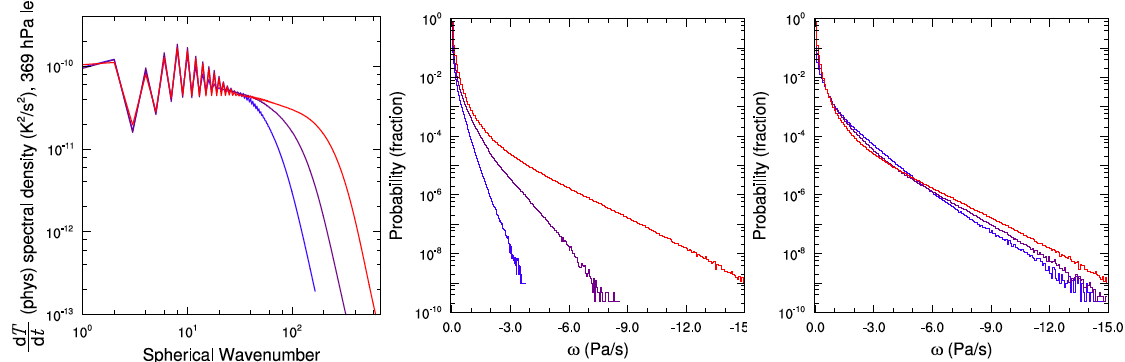
\includegraphics[width=30pc,angle=0]{figs/pg3panel.png}\\
\end{center}
\caption{(a) Wavenumber-power spectrum of the temperature tendencies from the moist physics, near the 369 hPa level, (b) probability density distribution and (c) the scaled probability density distribution of upward $\omega$ everywhere in the model, from three year long aqua-planet simulations at different grid resolutions.}
\label{fig:pg3panel}
\end{figure}

When the physics and dynamics grids are of a different resolution, it is not clear which grid determines the forcing scale. If the characteristic forcing scale is determined by the physics grid spacing, $\Delta x_{phys}$, than the $ne30pg2$ solution should more closely resemble the $ne20pg3$ solution, in which both the physics and dynamics grids are equal to the physics grid of $ne30pg2$. Likewise, if the dynamics grid spacing, $\Delta x_{dyn}$, governs the forcing scale than the $ne30pg2$ solution would more closely resemble the $ne30pg3$ solution. Figure \ref{fig:pg2panel}a is the  PDF of upward $\omega$ for simluations using the $ne20pg3$, $ne30pg2$ and $ne30pg3$ grids. It is clear that the $ne30pg2$ solution more closely resembles the $ne30pg3$ solution. Scaling the $ne30pg2$ PDF to the $ne30pg3$ grid using $\Delta x_{phys}$ overestimates the magnitude of $\omega$ in the $ne30pg3$ solution, whereas scaling the $ne20pg3$ solution to $ne30pg3$ does a fair job of predicting the $ne30pg3$ magnitudes (Figure \ref{fig:pg2panel}b). 

The dynamical core requires explicit numerical damping to increase with $\Delta x_{dyn}$ for numerical stability \citep{LetAl2018JAMES}. The hyper-viscosity coefficients are therefore smaller (and equal) in the $ne30pg2$ and $ne30pg3$ simulations, relative to the $ne20pg3$ simulation. Figure \ref{fig:pg2panel}a (green line) shows the PDF of upward $\omega$ for a $ne30pg2$ simulation, in which the hyper-viscosity coefficients are increased to $ne20pg3$ values (referred to as $ne30pg2-hivisc$). The solution now more closely resembles the $ne20pg3$ solution, indicating that an increase in explicit damping results in an increase in characteristic forcing scale. Through scaling the $ne30pg2-hivisc$ solutions to the $ne30pg3$ grid using $\Delta x_{phys}$, the scaled solution lie much closer to the $ne30pg3$ solution, compared wth scaling the default $ne30pg2$ solution using $\Delta x_{phys}$. When using a slightly lower resolution physics grid, $\Delta x_{phys}/\Delta x_{dyn} = 1.5$, it seems the forcing scale is primarily determined by $\Delta x_{dyn}$, due to $\Delta x_{dyn}$ dependent hyper-viscous damping.

\begin{figure}[t]
\begin{center}
\noindent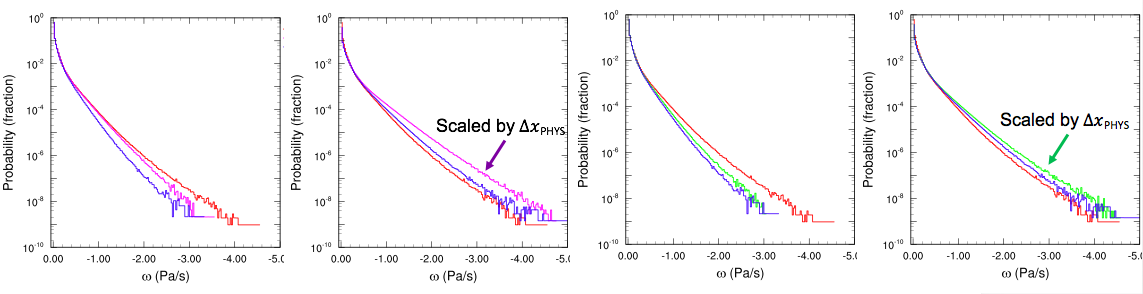
\includegraphics[width=30pc,angle=0]{figs/pdf-panel-hypervisc.png}\\
\end{center}
\caption{(a) Probability density distribution and (b) the scaled probability density distribution of upward $\omega$ everywhere in the model, from four different year long aqua-planet simulations at different grid resolutions. {\color{red}To do: make this a two panel plot with a clear legend.}}
\label{fig:pg2panel}
\end{figure}

The vertical velocity scale is determined by the characteristic forcing scale on the dynamical core grid. Mapping the physics forcing to the dynamics grid using a high-order reconstruction may introduce some fine scale features that the physics grid is unable to support, potentially increasing the vertical velocity scale. A $ne30pg2$ simulation using low-order reconstruction (bilinear interpolation from $pg2$ to $GLL$, and piecewise-constant mapping between $pg2$ and $CSLAM$ grids; referred to as $ne30pg2-loworder$) is carried out. The wave-number-power spectrum of the physics forcing in the upper-troposphere on the physics grid (Figure \ref{fig:loworder}a), and after the forcing is mapped to the dynamics grid (Figure \ref{fig:loworder}b) is provided for the $ne30pg2-loworder$, $ne30pg2$ and $ne30pg3$ simulations. 

On the physics grid, power at high wave-numbers is reduced in $ne30pg2-loworder$ compared with the default $ne30pg2$ solution, and both have less power than the $ne30pg3$ solution at most wave-numbers. On the dynamics grid, $ne30pg2-lowrder$ is the only solution with a clear reduction in power compared with $ne30pg3$ \textemdash the power spectrum of the $ne30pg2$ simulation is indistinguishable from the $ne30pg3$ solution at high wave-numbers (but note the damped oscillations in the $10-20$ wave-number window in $ne30pg2$). The PDFs of upward $\omega$ indicate the magnitude of the $ne30pg2$ solution lies intermediate to the two other simulations, but the magnitudes are closer to the $ne30pg3$ solution in the higher probability regions (greater than -2 hPa/day). High-order mapping is therefore an effective means to mitigate any reductions effective resolution arising from the use of a coarser physics grid.

\begin{figure}[t]
\begin{center}
\noindent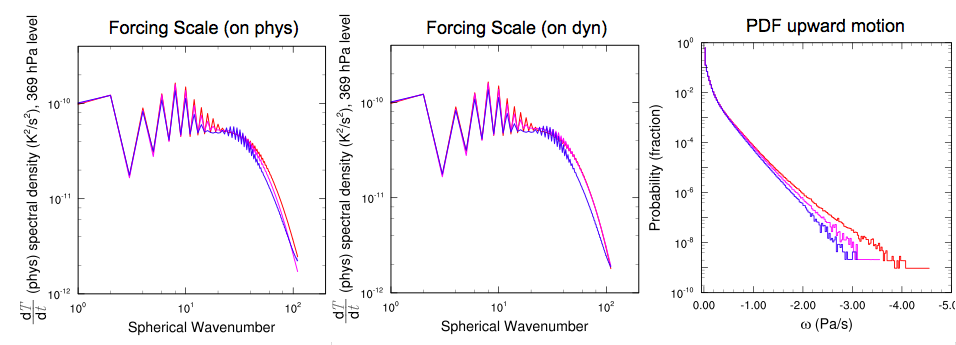
\includegraphics[width=30pc,angle=0]{figs/loworder-panel.png}\\
\end{center}
\caption{(a) Wavenumber-power spectrum of the temperature tendencies from the moist physics, near the 369 hPa level, on (a) the physics grid, and (b) the dynamics grid, and (c) the probability density distribution of upward $\omega$ everywhere in the model {\color{red}To do: make a clear legend.}}
\label{fig:loworder}
\end{figure}


\section{Conclusions}


%Text here ===>>>

%%

%  Numbered lines in equations:
%  To add line numbers to lines in equations,
%  \begin{linenomath*}
%  \begin{equation}
%  \end{equation}
%  \end{linenomath*}

%% Enter Figures and Tables near as possible to where they are first mentioned:
%
% DO NOT USE \psfrag or \subfigure commands.
%
% Figure captions go below the figure.
% Table titles go above tables;  other caption information
%  should be placed in last line of the table, using
% \multicolumn2l{$^a$ This is a table note.}
%
%----------------
% EXAMPLE FIGURE
%
% \begin{figure}[h]
% \centering
% when using pdflatex, use pdf file:
% \includegraphics[width=20pc]{figsamp.pdf}
%
% when using dvips, use .eps file:
% \includegraphics[width=20pc]{figsamp.eps}
%
% \caption{Short caption}
% \label{figone}
%  \end{figure}
%
% ---------------
% EXAMPLE TABLE
%
% \begin{table}
% \caption{Time of the Transition Between Phase 1 and Phase 2$^{a}$}
% \centering
% \begin{tabular}{l c}
% \hline
%  Run  & Time (min)  \\
% \hline
%   $l1$  & 260   \\
%   $l2$  & 300   \\
%   $l3$  & 340   \\
%   $h1$  & 270   \\
%   $h2$  & 250   \\
%   $h3$  & 380   \\
%   $r1$  & 370   \\
%   $r2$  & 390   \\
% \hline
% \multicolumn{2}{l}{$^{a}$Footnote text here.}
% \end{tabular}
% \end{table}

%% SIDEWAYS FIGURE and TABLE 
% AGU prefers the use of {sidewaystable} over {landscapetable} as it causes fewer problems.
%
% \begin{sidewaysfigure}
% \includegraphics[width=20pc]{figsamp}
% \caption{caption here}
% \label{newfig}
% \end{sidewaysfigure}
% 
%  \begin{sidewaystable}
%  \caption{Caption here}
% \label{tab:signif_gap_clos}
%  \begin{tabular}{ccc}
% one&two&three\\
% four&five&six
%  \end{tabular}
%  \end{sidewaystable}

%% If using numbered lines, please surround equations with \begin{linenomath*}...\end{linenomath*}
%\begin{linenomath*}
%\begin{equation}
%y|{f} \sim g(m, \sigma),
%\end{equation}
%\end{linenomath*}

%%% End of body of article

%%%%%%%%%%%%%%%%%%%%%%%%%%%%%%%%
%% Optional Appendix goes here
%
% The \appendix command resets counters and redefines section heads
%
% After typing \appendix
%
%\section{Here Is Appendix Title}
% will show
% A: Here Is Appendix Title
%
%\appendix

%\section{Here is a sample appendix}

%%%%%%%%%%%%%%%%%%%%%%%%%%%%%%%%%%%%%%%%%%%%%%%%%%%%%%%%%%%%%%%%
%
% Optional Glossary, Notation or Acronym section goes here:
%
%%%%%%%%%%%%%%  
% Glossary is only allowed in Reviews of Geophysics
%  \begin{glossary}
%  \term{Term}
%   Term Definition here
%  \term{Term}
%   Term Definition here
%  \term{Term}
%   Term Definition here
%  \end{glossary}

%
%%%%%%%%%%%%%%
% Acronyms
%   \begin{acronyms}
%   \acro{Acronym}
%   Definition here
%   \acro{EMOS}
%   Ensemble model output statistics 
%   \acro{ECMWF}
%   Centre for Medium-Range Weather Forecasts
%   \end{acronyms}

%
%%%%%%%%%%%%%%
% Notation 
%   \begin{notation}
%   \notation{$a+b$} Notation Definition here
%   \notation{$e=mc^2$} 
%   Equation in German-born physicist Albert Einstein's theory of special
%  relativity that showed that the increased relativistic mass ($m$) of a
%  body comes from the energy of motion of the body—that is, its kinetic
%  energy ($E$)—divided by the speed of light squared ($c^2$).
%   \end{notation}




%%%%%%%%%%%%%%%%%%%%%%%%%%%%%%%%%%%%%%%%%%%%%%%%%%%%%%%%%%%%%%%%
%
%  ACKNOWLEDGMENTS
%
% The acknowledgments must list:
%
% •	All funding sources related to this work from all authors
%
% •	Any real or perceived financial conflicts of interests for any
%	author
%
% •	Other affiliations for any author that may be perceived as
% 	having a conflict of interest with respect to the results of this
% 	paper.
%
% •	A statement that indicates to the reader where the data
% 	supporting the conclusions can be obtained (for example, in the
% 	references, tables, supporting information, and other databases).
%
% It is also the appropriate place to thank colleagues and other contributors. 
% AGU does not normally allow dedications.

%\acknowledgments

%% ------------------------------------------------------------------------ %%
%% Citations

% Please use ONLY \citet and \citep for reference citations.
% DO NOT use other cite commands (e.g., \cite, \citeyear, \nocite, \citealp, etc.).


%% Example \citet and \citep:
%  ...as shown by \citet{Boug10}, \citet{Buiz07}, \citet{Fra10},
%  \citet{Ghel00}, and \citet{Leit74}. 

%  ...as shown by \citep{Boug10}, \citep{Buiz07}, \citep{Fra10},
%  \citep{Ghel00, Leit74}. 

%  ...has been shown \citep [e.g.,][]{Boug10,Buiz07,Fra10}.



%%  REFERENCE LIST AND TEXT CITATIONS
%
% Either type in your references using
%
% \begin{thebibliography}{}
% \bibitem[{\textit{Kobayashi et~al.}}(2003)]{R2013} Kobayashi, T.,
% Tran, A.~H., Nishijo, H., Ono, T., and Matsumoto, G.  (2003).
% Contribution of hippocampal place cell activity to learning and
% formation of goal-directed navigation in rats. \textit{Neuroscience}
% 117, 1025--1035.
%
% \bibitem{}
% Text
% \end{thebibliography}
%
\bibliography{bib}
%%%%%%%%%%%%%%%%%%%%%%%%%%%%%%%%%%%%%%%%%%%%%%%
% Or, to use BibTeX:
%
% Follow these steps
%
% 1. Type in \bibliography{<name of your .bib file>} 
%    Run LaTeX on your LaTeX file.
%
% 2. Run BiBTeX on your LaTeX file.
%
% 3. Open the new .bbl file containing the reference list and
%   copy all the contents into your LaTeX file here.
%
% 4. Run LaTeX on your new file which will produce the citations.
%
% AGU does not want a .bib or a .bbl file. Please copy in the contents of your .bbl file here.


%% After you run BibTeX, Copy in the contents of the .bbl file here:


%%%%%%%%%%%%%%%%%%%%%%%%%%%%%%%%%%%%%%%%%%%%%%%%%%%%%%%%%%%%%%%%%%%%%
% Track Changes:
% To add words, \added{<word added>}
% To delete words, \deleted{<word deleted>}
% To replace words, \replace{<word to be replaced>}{<replacement word>}
% To explain why change was made: \explain{<explanation>} This will put
% a comment into the right margin.

%%%%%%%%%%%%%%%%%%%%%%%%%%%%%%%%%%%%%%%%%%%%%%%%%%%%%%%%%%%%%%%%%%%%%
% At the end of the document, use \listofchanges, which will list the
% changes and the page and line number where the change was made.

% When final version, \listofchanges will not produce anything,
% \added{<word or words>} word will be printed, \deleted{<word or words} will take away the word,
% \replaced{<delete this word>}{<replace with this word>} will print only the replacement word.
%  In the final version, \explain will not print anything.
%%%%%%%%%%%%%%%%%%%%%%%%%%%%%%%%%%%%%%%%%%%%%%%%%%%%%%%%%%%%%%%%%%%%%

%%%
\listofchanges
%%%

\end{document}

%%%%%%%%%%%%%%%%%%%%%%%%%%%%%%%%%%%%%
%% Supporting Information
%% (Optional) See AGUSuppInfoSamp.tex/pdf for requirements 
%% for Supporting Information.
%%%%%%%%%%%%%%%%%%%%%%%%%%%%%%%%%%%%%



%%%%%%%%%%%%%%%%%%%%%%%%%%%%%%%%%%%%%%%%%%%%%%%%%%%%%%%%%%%%%%%

More Information and Advice:

%% ------------------------------------------------------------------------ %%
%
%  SECTION HEADS
%
%% ------------------------------------------------------------------------ %%

% Capitalize the first letter of each word (except for
% prepositions, conjunctions, and articles that are
% three or fewer letters).

% AGU follows standard outline style; therefore, there cannot be a section 1 without
% a section 2, or a section 2.3.1 without a section 2.3.2.
% Please make sure your section numbers are balanced.
% ---------------
% Level 1 head
%
% Use the \section{} command to identify level 1 heads;
% type the appropriate head wording between the curly
% brackets, as shown below.
%
%An example:
%\section{Level 1 Head: Introduction}
%
% ---------------
% Level 2 head
%
% Use the \subsection{} command to identify level 2 heads.
%An example:
%\subsection{Level 2 Head}
%
% ---------------
% Level 3 head
%
% Use the \subsubsection{} command to identify level 3 heads
%An example:
%\subsubsection{Level 3 Head}
%
%---------------
% Level 4 head
%
% Use the \subsubsubsection{} command to identify level 3 heads
% An example:
%\subsubsubsection{Level 4 Head} An example.
%
%% ------------------------------------------------------------------------ %%
%
%  IN-TEXT LISTS
%
%% ------------------------------------------------------------------------ %%
%
% Do not use bulleted lists; enumerated lists are okay.
% \begin{enumerate}
% \item
% \item
% \item
% \end{enumerate}
%
%% ------------------------------------------------------------------------ %%
%
%  EQUATIONS
%
%% ------------------------------------------------------------------------ %%

% Single-line equations are centered.
% Equation arrays will appear left-aligned.

Math coded inside display math mode \[ ...\]
 will not be numbered, e.g.,:
 \[ x^2=y^2 + z^2\]

 Math coded inside \begin{equation} and \end{equation} will
 be automatically numbered, e.g.,:
 \begin{equation}
 x^2=y^2 + z^2
 \end{equation}


% To create multiline equations, use the
% \begin{eqnarray} and \end{eqnarray} environment
% as demonstrated below.
\begin{eqnarray}
  x_{1} & = & (x - x_{0}) \cos \Theta \nonumber \\
        && + (y - y_{0}) \sin \Theta  \nonumber \\
  y_{1} & = & -(x - x_{0}) \sin \Theta \nonumber \\
        && + (y - y_{0}) \cos \Theta.
\end{eqnarray}

%If you don't want an equation number, use the star form:
%\begin{eqnarray*}...\end{eqnarray*}

% Break each line at a sign of operation
% (+, -, etc.) if possible, with the sign of operation
% on the new line.

% Indent second and subsequent lines to align with
% the first character following the equal sign on the
% first line.

% Use an \hspace{} command to insert horizontal space
% into your equation if necessary. Place an appropriate
% unit of measure between the curly braces, e.g.
% \hspace{1in}; you may have to experiment to achieve
% the correct amount of space.


%% ------------------------------------------------------------------------ %%
%
%  EQUATION NUMBERING: COUNTER
%
%% ------------------------------------------------------------------------ %%

% You may change equation numbering by resetting
% the equation counter or by explicitly numbering
% an equation.

% To explicitly number an equation, type \eqnum{}
% (with the desired number between the brackets)
% after the \begin{equation} or \begin{eqnarray}
% command.  The \eqnum{} command will affect only
% the equation it appears with; LaTeX will number
% any equations appearing later in the manuscript
% according to the equation counter.
%

% If you have a multiline equation that needs only
% one equation number, use a \nonumber command in
% front of the double backslashes (\\) as shown in
% the multiline equation above.

% If you are using line numbers, remember to surround
% equations with \begin{linenomath*}...\end{linenomath*}

%  To add line numbers to lines in equations:
%  \begin{linenomath*}
%  \begin{equation}
%  \end{equation}
%  \end{linenomath*}



